\documentclass[a4paper]{report}
\usepackage{setspace}
%\usepackage{subfigure}

\usepackage{tikz}
\pagestyle{plain}
\usepackage{amssymb,graphicx,color}
\usepackage{amsfonts}
\usepackage{latexsym}
\usepackage{amsmath}
\usepackage{graphicx}
\usepackage{appendix}
\usepackage{stfloats}
\usepackage{subfig}
\usepackage{algorithm}
\usepackage{algpseudocode}
\usepackage[a4paper, margin = 3cm, bottom = 2.5cm]{geometry}
\usepackage{booktabs}
\usepackage{titlesec}
\usepackage{pgfplotstable}
\usepackage{booktabs}


\titleformat{\chapter}[hang]
  {\normalfont\huge\bfseries}
  {\thechapter}{1em}{}

\titlespacing*{\chapter}
  {0pt}{0pt}{20pt}

\usepackage{xcolor}

\newtheorem{theorem}{THEOREM}
\newtheorem{lemma}[theorem]{LEMMA}
\newtheorem{corollary}[theorem]{COROLLARY}
\newtheorem{proposition}[theorem]{PROPOSITION}
\newtheorem{remark}[theorem]{REMARK}
\newtheorem{definition}[theorem]{DEFINITION}
\newtheorem{fact}[theorem]{FACT}

\newtheorem{problem}[theorem]{PROBLEM}
\newtheorem{exercise}[theorem]{EXERCISE}
\def \set#1{\{#1\} }

\newenvironment{proof}{
PROOF:
\begin{quotation}}{
$\Box$ \end{quotation}}



\newcommand{\nats}{\mbox{\( \mathbb N \)}}
\newcommand{\rat}{\mbox{\(\mathbb Q\)}}
\newcommand{\rats}{\mbox{\(\mathbb Q\)}}
\newcommand{\reals}{\mbox{\(\mathbb R\)}}
\newcommand{\ints}{\mbox{\(\mathbb Z\)}}

%%%%%%%%%%%%%%%%%%%%%%%%%%


\title{{\vspace{-10em} \includegraphics[scale=0.4]{}}\\
{{\Huge A Diagrammatic and Categorical Implementation of Counterfactual Identifiability}}\\
}
\date{Submission date: 24 04 2026}
\author{Candidate number: RTCG5\thanks{
{\bf Disclaimer:}
This report is submitted as part requirement for the MEng at UCL. It is
substantially the result of my own work except where explicitly indicated in the text.
The report will be distributed to the internal and external examiners, but thereafter may not be copied or distributed except with permission from the author.}
\\ \\
Year 4 MEng Computer Science\\ \\
Supervisor: Prof Fabio Zanasi}


\begin{document}
 
\onehalfspacing

\maketitle
\begin{abstract}
This project presents a diagrammatic and categorical implementation of counterfactual identifiability analysis, with the goal of bridging the gap between symbolic causal inference algorithms and compositional semantic representations. The system implements a complete end-to-end pipeline, including ADMG compilation, parallel-world construction, counterfactual simplification, recursive identification via R-fragment decomposition, and final probability expression reconstruction. Causal models are represented as wiring diagrams using the Catlab framework, enabling the identification process to be interpreted as a sequence of compositional diagram transformations instead of purely symbolic manipulations. Correctness is validated through unit testing and cross-tool comparison with the \texttt{cfid} package in R, demonstrating semantic consistency across all identifiable cases. Experimental evaluation further shows that the proposed implementation achieves competitive and often superior runtime performance, particularly on larger and sparser graphs, by shifting computational effort into an explicit simplification stage. In addition to performance, the framework provides improved interpretability by exposing intermediate diagrammatic structures throughout the pipeline (implemented by \texttt{Chyp}). These visualisations make the internal reasoning process transparent and facilitate debugging and analysis. Overall, this project demonstrates that counterfactual identification can be effectively implemented as a compositional diagram transformation system, providing a faithful, interpretable, and efficient computational realisation of existing causal inference theory.
\end{abstract}
\tableofcontents
\setcounter{page}{1}


\chapter{Introduction}
Causal reasoning provides a formal framework for understanding cause–effect relationships in complex systems. Broadly, research in this area can be divided into two main branches: causal discovery, which aims to learn causal structure from data, and causal inference, which focuses on estimating the effects of interventions. The modern formulation of this framework originates from the work of Judea Pearl and his collaborators, where causal assumptions are encoded using directed acyclic graphs (DAGs) and Structural Causal Models (SCMs). Within this framework, probabilistic reasoning and graph structures together determine which causal queries can be identified from observational or experimental data.

One of the central theoretical questions in this area is identifiability: given a causal graph and a set of available distributions (observational or interventional), can a target causal or counterfactual query be uniquely determined? For the identification of causal effects, Shpitser and Pearl \cite{shpitser2008complete} provided a complete characterisation, including both a graphical criterion describing when identification is impossible and a correct and complete identification algorithm (the ID algorithm). This theory was subsequently extended to counterfactual queries, leading to the development of the ID-CF algorithm, which determines when a counterfactual probability can be computed from experimental distributions.

In practice, identification algorithms are typically implemented in a symbolic form. For example, the cfid package in R implements the ID-CF algorithm and outputs the corresponding algebraic probability expressions. Although such implementations are computationally correct, they largely operate at the level of symbolic manipulation. Graph simplification, recursive decomposition into F-fragments, graph-structural transformations, and expression reduction steps are performed internally, yet without explicit structural interpretation. As a result, the algorithm appears as a sequence of algebraic rewriting rules rather than a transparent process of structural transformation.

At the same time, category theory provides a compositional and graphical foundation for probabilistic reasoning. Probability theory can be formalized within the framework of Markov categories or cd-categories, where stochastic processes are modeled as morphisms in a symmetric monoidal category equipped with copying and discarding structure (Fritz, 2020; Jacobs, 2019). Within this framework, reasoning is carried out using string diagrams, offering a graphical calculus that is both intuitive and formally rigorous.

Building on the diagrammatic approach to causal inference introduced by Jacobs, Kissinger, and Zanasi~\cite{jacobs2019causal, DBLP:journals/mscs/JacobsKZ21}, causal models can be given a string-diagrammatic formalisation in which DAGs correspond one-to-one with network diagrams, structural causal models are interpreted as stochastic morphisms in a cd-category, and interventions are represented as “surgical” transformations of diagrams. This perspective has been further developed and reformulated by Lorenz and Tull~\cite{lorenz2023causal}. Within this framework, both causal effect and counterfactual identification problems can be expressed directly in graphical language. This viewpoint suggests that identification algorithms admit a deeper structural interpretation: rather than treating ID-CF as a purely symbolic procedure, its recursive steps may be understood as compositional diagram transformations in a symmetric monoidal category. Accordingly, the central research question of this project is: How the complete theory of counterfactual identification can be realized as a modular and computationally faithful diagram transformation system that bridges symbolic identification algorithms and compositional categorical semantics.

To implement this framework, we employ the Catlab.jl ecosystem in Julia. Catlab provides a formal infrastructure for working with wiring diagrams and symmetric monoidal categories, allowing causal structures to be represented directly as compositional diagrammatic objects. Julia’s multiple-dispatch paradigm and strong support for symbolic computation facilitate a modular implementation of recursive identification algorithms. The choice of this environment ensures that the computational realisation remains faithful to the underlying categorical semantics, rather than merely serving as a symbolic rewriting system.

To support structural inspection and verification of diagrammatic transformations, the intermediate results of the identification pipeline are exported to the Chyp proof assistant. Chyp is an interactive theorem-proving environment for string diagrams, designed for compositional reasoning in symmetric monoidal categories. By rendering each major stage of the algorithm as a diagram in Chyp, the recursive structure of identification becomes visually explicit. This integration enables not only visualisation but also structural validation of diagrammatic rewrites, reinforcing the alignment between symbolic identification theory and categorical semantics.

The objectives of this project are as follows:

\begin{itemize}
    \item To implement a diagrammatic representation of causal models and counterfactual queries using Catlab wiring diagrams.
    \item To realise the main stages of the ID-CF pipeline, including ADMG compilation, parallel-world construction, counterfactual simplification, R-fragment decomposition, and expression reconstruction.
    \item To provide visualisation support for intermediate diagrammatic structures using Chyp.
    \item To validate the implementation through unit tests and comparison with the existing \texttt{cfid} package.
    \item To evaluate the runtime behaviour of the implementation on benchmark examples and synthetic graph structures.
\end{itemize}


\chapter{context}
\section{Structural Causal Models (SCMs)}
Structural Causal Models (SCMs), introduced by Judea Pearl\cite{pearl2009causality}, provide a formal framework for representing causal relationships between variables. An SCM consists of a set of structural equations together with a directed graph that captures the dependencies between variables. In this framework, each variable is determined by a function of its parent variables and an associated exogenous noise variable. The graphical structure of the model therefore encodes the causal mechanisms that generate the observed data.

Formally, a structural causal model can be defined as a tuple
\[
M = (U, V, F, P(U))
\]
where:

\begin{itemize}
\item $U$ denotes the set of exogenous variables.
\item $V$ denotes the set of endogenous variables.
\item $F$ is a collection of structural functions that determine how each variable in $V$ is generated from its parent variables.
\item $P(U)$ is a probability distribution over the exogenous variables.
\end{itemize}

Through the structural equations and the propagation of exogenous randomness, the model induces a joint probability distribution over the endogenous variables.

The causal structure of an SCM is typically represented using a 
\textbf{Directed Acyclic Graph (DAG)} . In such a graph, nodes correspond to variables and directed edges represent direct causal relationships between them. The graph encodes conditional independence relations via the criterion of d-separation \cite{geiger1990dseparation}. Moreover, the acyclicity property ensures that the structural equations can be evaluated in a topological order, allowing the model to generate a well-defined joint probability distribution over all variables.

DAGs therefore provide an intuitive graphical representation of causal mechanisms while maintaining a precise mathematical semantics.

Moreover, an important feature of structural causal models is their ability to represent \textbf{interventions}. An intervention refers to an external operation in which a variable is deliberately set to a specific value manually, rather than being generated through the natural causal mechanisms of the system.

Within the framework of structural causal models, interventions are represented using the \textbf{do-operator}\cite{10.1093/biomet/82.4.669}. The expression $do(X = x)$ denotes that the variable $X$ is actively set to the value $x$. When such an intervention occurs, the original causal mechanism that determines $X$ is removed. From the perspective of structural equations, this corresponds to replacing the structural equation for $X$ with a fixed assignment, that is, directly setting $X = x$. From the perspective of graphical models, this operation can be understood as deleting all incoming edges pointing to X in the causal graph. After the intervention, the value of X is no longer determined by its original parent nodes, but is directly specified by external manipulation.

After performing an intervention, the model induces an \textbf{interventional distribution}, denoted by
\[
P(Y \mid do(X = x)).
\]
This distribution represents the probability distribution of the variable $Y$ when the variable $X$ is forcibly set to the value $x$. It is important to note that this distribution is different from the conditional probability $P(Y \mid X = x)$. The conditional probability only describes the distribution of $Y$ in observational data where $X$ happens to take the value $x$, and therefore reflects statistical correlation. In contrast, the interventional distribution describes how $Y$ would change if we actively manipulate the value of $X$, and thus captures the \textbf{causal effect} of $X$ on $Y$.

While the do-operator provides a formal semantics for causal interventions, in many practical situations the quantities expressed using the do-operator cannot be directly measured. This leads to the central question of \textbf{identifiability} in causal inference.

Identifiability is a core concept in causal reasoning. 
In many real-world problems, interventional distributions cannot be obtained directly through experiments, since performing actual interventions may be costly, ethically unacceptable, or simply infeasible. 
As a result, researchers often only have access to \textbf{observational data}.In such situations, a key question arises: whether a causal effect can be computed using observational data alone.

The answer is yes. Formally, a causal query is said to be \textbf{identifiable} if it can be uniquely expressed as a function of the observational distribution. 
In other words, even if we do not actually perform the intervention, we may still be able to compute the corresponding interventional distribution provided that the causal graph and the observational data contain sufficient information.

For example, suppose we are interested in studying the causal effect of a variable $X$ on another variable $Y$. 
Ideally, we would like to compute the quantity
\[
P(Y \mid do(X = x)),
\]
which represents the distribution of $Y$ when we actively set $X$ to the value $x$. 
However, when only observational data are available, the quantity we can observe is typically the joint distribution over all variables in the system, denoted by $P(V)$. 
Therefore, the \textbf{identification problem} asks whether the causal query $P(Y \mid do(X = x))$ can be expressed purely in terms of the observational distribution.

In some cases, this can be achieved easily. 
For example, if there are no confounding variables that simultaneously influence both $X$ and $Y$, then the causal effect reduces to a simple conditional probability:
\[
P(Y \mid do(X = x)) = P(Y \mid X = x).
\]
However, the situation becomes more complicated when hidden confounders are present. In such cases, determining whether the causal effect can still be computed from observational data becomes a non-trivial problem. To address this problem, researchers have proposed a series of \textbf{identification algorithms}. Among the most well-known are the \textbf{ID algorithm}\cite{pearl2009causality}, and its later extension to counterfactual queries, the \textbf{ID-CF algorithm}\cite{shpitser2008complete}. These algorithms provide systematic procedures for determining whether a given causal query is identifiable, and, when it is identifiable, for deriving an expression that depends only on observable distributions. This will be discussed in detail in a later section.

\section{Counterfactual}
To further develop the discussion, it is necessary to introduce an important concept: \textbf{counterfactuals}. Counterfactual reasoning concerns the analysis of questions of the form “what would have happened if things had been different”. Such questions describe hypothetical scenarios that did not actually occur in reality, but for which we wish to infer how the outcome would change if certain conditions were altered.\cite{pearl2009causality, shpitser2007counterfactuals}

Counterfactual questions are very common in the real world, especially when we aim to understand the impact of an action or decision. For example, suppose a patient did not receive a particular treatment and ultimately did not recover. A natural question to ask is: if the patient had received the treatment, would the patient have recovered? This question describes a scenario that did not actually occur and therefore constitutes a counterfactual query. The process of reasoning about such hypothetical scenarios is referred to as \textbf{counterfactual reasoning}.

In structural causal bfmodels, counterfactual reasoning is represented using \textbf{counterfactual variables}. A counterfactual variable describes the value that a variable would take under a particular hypothetical intervention. Formally, the counterfactual variable $Y_x$ denotes the value that $Y$ would take if we were to intervene on the variable $X$ and set it to the value $x$. 
This notation allows us to clearly distinguish between the value of a variable that is actually observed in reality and the value that it would take under a hypothetical intervention.

Continuing with the previous example, suppose that $X$ represents whether a patient receives a treatment and $Y$ represents whether the patient recovers. Then $Y_1$ denotes whether the patient would recover if the patient received the treatment, while $Y_0$ denotes whether the patient would recover if the patient did not receive the treatment. In practice, however, for any individual we can only observe one of these outcomes. 
If the patient receives the treatment, we can observe $Y_1$, but $Y_0$ remains unobserved. Conversely, if the patient does not receive the treatment, we can observe $Y_0$, while $Y_1$ is unknown.

Structural causal models provide a formal framework that allows us to reason about counterfactual variables even when it is impossible to observe all counterfactual outcomes simultaneously. Through structural equations and causal graphs, the model captures the causal relationships among variables, enabling us to analyse the outcomes that may arise under different intervention scenarios.

Once counterfactual variables have been defined, it becomes natural to ask probabilistic questions about them. Such questions are known as \textbf{counterfactual queries}.

\textbf{Counterfactual queries} concern the probabilities of outcomes under hypothetical intervention scenarios. While the counterfactual variables introduced in the previous section describe the value that a single variable would take under a particular intervention, counterfactual queries focus on the probability distributions of such variables. One of the simplest forms of a counterfactual query is
\[
P(Y_x = y),
\]
which represents the probability that the variable $Y$ would take the value $y$ if the variable $X$ were set to $x$ through an intervention. 

More complex counterfactual queries may additionally incorporate observational information from the real world. A useful example involves three variables. Suppose $Z$ represents a patient's underlying health condition, $X$ represents whether the patient receives a treatment, and $Y$ represents whether the patient recovers. The variable $Z$ may influence both the treatment decision and the recovery outcome.

In this setting, a simple counterfactual query is
\[
P(Y_x = y),
\]
which asks for the probability that the patient would recover if the treatment were set to $x$.

More complex counterfactual queries may incorporate observational evidence. For instance,
\[
P(Y_x = y \mid X = x'),
\]
asks the following question: given that the patient actually received treatment $x'$, what would the recovery outcome have been if the treatment had instead been set to $x$?

Even richer queries may condition on additional observed variables, such as
\[
P(Y_x = y \mid X = x', Z = z).
\]

In this case, the variables $X = x'$ and $Z = z$ refer to information observed in the actual world, while the counterfactual variable $Y_x$ refers to a hypothetical world in which the treatment is set to $x$. Therefore, the expression simultaneously involves observed information and a hypothetical intervention.

This illustrates the \textbf{multiple worlds structure} of counterfactual reasoning. Observed variables such as $X$ and $Z$ describe the actual world, while counterfactual variables such as $Y_x$ correspond to alternative worlds generated by interventions.

The counterfactual variables and counterfactual queries introduced above naturally lead to an important problem known as the \textbf{counterfactual identification problem}. In many practical situations, it is impossible to directly observe the outcomes under hypothetical interventions, since performing real interventions may be costly, infeasible, or ethically unacceptable. Thus, we typically only have access to \textbf{observational data} together with causal structural assumptions encoded by a causal graph.

The counterfactual identification problem can be stated as follows: given a causal graph and the observational distribution of the system variables, can we compute the probability of a counterfactual query?

More specifically, suppose we are given a causal model described by a causal graph $G$, and we can observe the joint distribution $P(V)$ over a set of system variables $V$. 
For a counterfactual query such as
\[
P(Y_x \mid e),
\]
where $e$ denotes observed evidence, the identification problem asks whether this quantity can be uniquely expressed as a function of the observational distribution.

In some cases, this is indeed possible. The structure of the causal graph may provide sufficient information to express the counterfactual quantity in terms of observable probabilities. However, in other cases the available information is insufficient, and the counterfactual query cannot be determined from observational data alone.

Determining whether a counterfactual query is identifiable, and deriving the corresponding expression when identification is possible, is a central problem in causal inference. To address this problem, a number of algorithmic methods have been developed. Among them, the \textbf{ID-CF algorithm}\cite{shpitser2008complete} provides a systematic procedure for determining whether a counterfactual query is identifiable and, whenever possible, deriving an equivalent expression in terms of observable distributions.

In this project, I study how the counterfactual identification process can be interpreted and implemented using compositional diagrammatic structures.

\section{Diagrammatic Semantics of Causality}
\subsection{String Diagrams}
To introduce the categorical framework used in this project, we briefly review \textbf{string diagrams} \cite{intro_to_string_diagram}. String diagrams provide a graphical syntax for morphisms in monoidal categories and are widely used to describe compositional systems \cite{Selinger2011}. Compared with purely symbolic notation, they offer an intuitive way to visualise how different components interact and how information flows through a system.

In this graphical language, \textbf{wires} represent objects such as variables or 
probability spaces, while \textbf{boxes} represent morphisms, which may correspond 
to transformations, stochastic mechanisms, or conditional relationships between 
variables. Composition of morphisms is represented by connecting wires. 
Sequential composition is depicted by stacking boxes vertically, while parallel 
composition is represented by placing boxes side by side.

\paragraph{Morphisms}

Consider a morphism $f$ with one input wire $A$ and two output wires $B$ and $C$:

\[
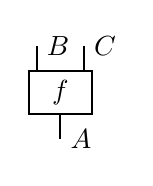
\begin{tikzpicture}[thick, baseline=(box.base)]
\node[draw, minimum width=0.8cm, minimum height=0.5cm] (box) {$f$};
\draw (box.south) -- ++(0,-0.3) node[right] {$A$};
\draw (box.north) ++(-0.3,0) -- ++(0,0.3) node[right] {$B$};
\draw (box.north) ++(0.3,0) -- ++(0,0.3) node[right] {$C$};
\end{tikzpicture}
\]

In probabilistic terms, such a morphism can be interpreted as a \textbf{channel}, corresponding to a conditional probability distribution \cite{markov-kernel-cat, cho2019disintegration}. More precisely, it represents a conditional probability distribution that describes the joint distribution of $B$ and $C$ conditioned on the input variable $A$, which can be written as $P(B,C \mid A)$. Intuitively, the box represents a stochastic process that generates outputs $B$ and $C$ from the input $A$.

\paragraph{Sequential Composition}

If $f : A \rightarrow B$ and $g : B \rightarrow C$ are two morphisms, their 
sequential composition $g \circ f$ corresponds to applying $f$ first and then 
$g$. In a string diagram this is represented by connecting the output wire of 
$f$ to the input wire of $g$:

\begin{center}
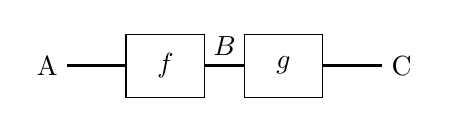
\begin{tikzpicture}
\node (A) at (0,0) {A};
\node[draw, rectangle, minimum width=1cm, minimum height=0.8cm] (F) at (1.5,0) {$f$};
\node[draw, rectangle, minimum width=1cm, minimum height=0.8cm] (G) at (3,0) {$g$};
\node (C) at (4.5,0) {C};
\draw[thick] (A) -- (F) -- (G) -- (C);
\node[above] at (2.25,0) {$B$};
\end{tikzpicture}
\end{center}

This diagram expresses the flow of information from $A$ through the intermediate 
variable $B$ and finally to $C$.

\paragraph{Parallel Composition}

When two morphisms operate independently on different inputs, they can be 
composed in parallel. For example, if $f : A \rightarrow B$ and $g : C \rightarrow D$, 
their parallel composition is represented by placing the two boxes next to each 
other:

\begin{center}
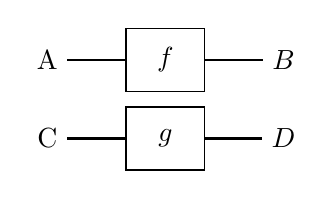
\begin{tikzpicture}
\node (A) at (0,1) {A};
\node[draw, rectangle, minimum width=1cm, minimum height=0.8cm] (F) at (1.5,1) {$f$};
\node (B) at (3,1) {$B$};

\node (C) at (0,0) {C};
\node[draw, rectangle, minimum width=1cm, minimum height=0.8cm] (G) at (1.5,0) {$g$};
\node (D) at (3,0) {$D$};

\draw[thick] (A) -- (F) -- (B);
\draw[thick] (C) -- (G) -- (D);
\end{tikzpicture}
\end{center}

Parallel composition represents independent transformations occurring simultaneously on different variables.

These graphical composition rules allow complex processes to be constructed from simpler components. In the context of causal modelling, they provide a natural way to represent how variables interact and how causal mechanisms can be composed to form larger systems.

\subsection{SMC}

The graphical language of string diagrams is mathematically grounded in the theory of \textbf{Symmetric Monoidal Categories} (SMCs)\cite{Selinger2011}. Symmetric monoidal categories provide an abstract mathematical framework for describing systems composed of multiple interacting processes.

In category theory, a category consists of two fundamental components: \textbf{objects} and \textbf{morphisms} between objects\cite{basic-cat-theory}. Morphisms can be understood as transformations or processes that map one object to another. When the output type of one morphism matches the input type of another, the two morphisms can be combined through an operation known as \textbf{composition}. 
Intuitively, this corresponds to the sequential execution of processes.

A monoidal category further introduces an additional operation known as the \textbf{tensor product}. The tensor product allows two objects or two morphisms to be combined, thereby representing the parallel structure of two systems. For example, if $A$ and $B$ are two objects, then $A \otimes B$ denotes the joint system composed of these two objects. If $f : A \rightarrow B$ and $g : C \rightarrow D$ are two morphisms, then $f \otimes g$ represents two processes acting on different systems and occurring simultaneously.

Another important property of symmetric monoidal categories is \textbf{symmetry}. This property allows the order of objects in a tensor product to be exchanged, meaning that $A \otimes B$ and $B \otimes A$ are structurally equivalent. 

String diagrams provide a natural graphical representation of these structures. In a string diagram, sequential composition corresponds to connecting boxes vertically, while the tensor product corresponds to placing boxes side by side. The symmetry operation is represented by crossing wires. In this way, string diagrams can be understood as a graphical syntax for symmetric monoidal categories. 
Rather than using complex symbolic expressions to represent tensor products and compositions, the same mathematical structures can be expressed directly through transformations of diagrams.

This graphical perspective is particularly useful in probabilistic modelling and causal reasoning, where complex systems are often constructed by combining multiple simple mechanisms. Symmetric monoidal categories provide the mathematical foundation for this compositional structure and form the theoretical basis for the semantic interpretation of causal diagrams.

\subsection{Markov Categories}

Markov categories\cite{FRITZ2020107239} extend symmetric monoidal categories by introducing additional structure that captures probabilistic behaviour such as copying and discarding random variables.

Although symmetric monoidal categories provide a general mathematical framework for describing compositional systems, additional structure is required to capture probabilistic processes. Markov categories extend symmetric monoidal categories with structures that describe probabilistic behaviour, allowing stochastic processes to be formalised within a categorical setting. 
In a Markov category, objects typically represent random variables or probability spaces, while morphisms represent stochastic maps, also known as Markov kernels \cite{markov-kernel-cat}. Intuitively, a morphism from an object $A$ to an object $B$ can be interpreted as a conditional probability distribution describing how the random variable $B$ depends on the random variable $A$.

A key feature of Markov categories is the so-called \textbf{copy–discard structure}, often abbreviated as \textbf{CDU}\cite{stoch-cdu}. This structure introduces two fundamental operations corresponding to important computational processes in probability theory.

\begin{itemize}

\item \textbf{Copy}.  
The copy operation duplicates an object, allowing the same piece of information to be used in multiple parts of a causal or probabilistic computation. 
In string diagrams this operation is represented by a branching wire, indicating that a variable is copied into two identical outputs. 
Formally, this corresponds to a morphism
\[
A \to A \otimes A .
\]
Graphically, it is depicted as
(\begin{tikzpicture}[thick, baseline=(box.base), scale=0.5]
\node[draw, circle, fill=black, minimum size=4pt, inner sep=0pt] (copy) at (0,0) {};
\draw (copy) -- ++(45:1) node[right] {$A$};
\draw (copy) -- ++(135:1) node[right] {$A$};
\draw (copy) -- ++(270:1) node[right] {$A$};
\end{tikzpicture}).

\item \textbf{Discard}.  
The discard operation represents the ability to ignore or remove a variable from the system. 
From a probabilistic perspective, this corresponds to marginalisation, where a variable is integrated out while leaving the remaining variables unchanged. 
Formally, discard is a morphism
\[
A \to I ,
\]
where $I$ denotes the monoidal unit. 
In a string diagram this is represented by a wire terminating at a special node:
\[
\big(\:
\begin{tikzpicture}[thick, baseline=(box.base), scale=0.7]
\node[draw, circle, fill=black, minimum size=4pt, inner sep=0pt] (discard) at (0,0.2) {};
\draw (0,-0.2) -- (discard);
\node[right] {$A$};
\end{tikzpicture}
: A \to I
\:\big).
\]

\item \textbf{Uniform}.  
The uniform operation introduces a state that is generated independently of any prior input. 
Intuitively, it corresponds to sampling a variable from a default distribution, which is useful when modelling interventions that set a variable independently of the rest of the system. 
This operation is represented by a morphism
\[
I \to A .
\]
In the graphical language it is depicted as
(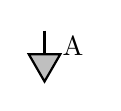
\begin{tikzpicture}[thick, scale=0.1, baseline=(current bounding box.center)]
\coordinate (A) at (0,2);
\coordinate (B) at (4,2);
\coordinate (C) at (2,-1.464);

\fill[gray!50] (A) -- (B) -- (C) -- cycle;
\draw (A) -- (B) -- (C) -- cycle;
\draw (2,5) -- (2,2);
\node[right] at (3,3) {A};
\end{tikzpicture}
: I \to A).
    
\end{itemize}

\section{Categorical Implementation Tools}
To implement the diagrammatic causal framework proposed in this work, we make use of the Julia programming language together with tools from the AlgebraicJulia ecosystem. 
These tools provide the necessary computational support for categorical modelling and diagrammatic reasoning.

Julia is a modern programming language designed for scientific computing. It combines a concise and expressive syntax with high execution efficiency, making it well suited for implementing complex mathematical structures and algorithmic models. In particular, Julia’s type system and multiple dispatch mechanism allow abstract objects such as categories, morphisms, and graph structures to be represented in a natural and flexible way within programs.

Building on this foundation, the AlgebraicJulia project provides a collection of Julia libraries designed for \textbf{Applied Category Theory}. These libraries allow many mathematical structures from category theory to be directly represented and manipulated within programs. Among these tools, \textbf{Catlab} is the central library used in this project. Catlab provides a computational framework for constructing and working with categorical structures. It supports the representation of objects, morphisms, functors, and various graph-based structures, making it well suited for describing complex compositional systems.

One of the key features of Catlab is its support for \textbf{wiring diagrams}. Catlab represents causal structures using wiring diagrams, which provide a computational realisation of symmetric monoidal categories \cite{patterson2020wiring}. Wiring diagrams represent a system as a composition of multiple components, where each component corresponds to a transformation and the connections between components are represented by wires that indicate the flow of information.

This representation aligns naturally with causal models. In a structural causal model, each mechanism can be interpreted as a morphism, while dependencies between variables correspond to wires in the diagram. By composing these elements, Catlab allows causal systems to be represented as structured diagrams rather than purely symbolic expressions. Another advantage is that Catlab preserves the categorical semantics of the models. Operations performed on diagrams correspond directly to well-defined categorical transformations. This ensures that the computational implementation remains faithful to the underlying mathematical theory.

For these reasons, Catlab provides an effective and flexible platform for implementing the diagrammatic causal framework used in this project.

\section{Diagrammatic Reasoning Tool}
In addition to implementing categorical models, this project also makes use of Chyp, a graphical proof assistant designed for reasoning with string diagrams.

Chyp provides an interactive environment for constructing, visualising, and transforming string diagrams. It is particularly useful for working with diagrammatic calculi arising from monoidal categories. Rather than manipulating symbolic expressions, users can perform reasoning steps directly on graphical representations of diagrams. One of the main capabilities of Chyp is graphical rewriting. iagrammatic rewriting rules allow diagrams to be transformed while preserving their semantic meaning. These transformations correspond to algebraic identities in the underlying categorical framework. By applying rewriting rules, complex diagrammatic expressions can be simplified or normalised.

This graphical rewriting mechanism is closely related to the process of diagrammatic reasoning used in categorical approaches to causality. Many causal transformations can be interpreted as structural modifications of diagrams. As a result, tools such as Chyp provide a natural way to visualise and verify these transformations.

In this project, Chyp is used to visualise intermediate structures produced by the causal algorithms. In particular, the outputs of the main procedures—such as \textbf{admg-compile}, \textbf{simplify-cf}, and \textbf{id-cf} can be exported as diagrams and inspected using Chyp. This allows the structural transformations performed by the algorithms to be examined in a graphical form.

By combining Catlab for computational modelling and Chyp for graphical reasoning, the project establishes a workflow that connects categorical theory, algorithmic implementation, and visual verification.

\chapter{Methodology}
This chapter presents the methodological framework used in this work to implement the counterfactual identification algorithm. 
The framework approaches counterfactual identification from a diagrammatic and categorical perspective, transforming counterfactual queries into probability expressions that can be evaluated from observational data.

The inputs to this method consist of two main components. The first component is a \textit{causal graph}, which describes the structural relationships among variables. The graph represents the underlying structural causal model and may contain both directed edges and bi-directed edges, where bi-directed edges indicate dependencies arising from latent confounding variables. The second component is a \textbf{counterfactual query}, which can typically be written in the form
\[
P(Y_x \mid e),
\]
where $Y_x$ denotes the value of the variable $Y$ under the intervention $do(X=x)$, and $e$ represents observed evidence.

Given these inputs, the goal of the framework is to determine whether the counterfactual query is \textbf{identifiable}. 
If the query is identifiable, the framework further derives an equivalent probabilistic expression that depends only on observable or interventional distributions. Therefore, the output of the system is a probabilistic expression. When identification succeeds, this expression is composed entirely of observational or interventional probabilities, allowing it to be directly evaluated from available data. If the query is not identifiable, the algorithm returns a failure indicating that the desired counterfactual quantity cannot be determined from the given information.

The method implemented in this work is grounded in several classical theoretical frameworks from causal inference. 
In particular, it draws on the \textbf{ID algorithm} \cite{shpitser2006identification}, which is used for identifying causal effects; the \textbf{IDC algorithm} \cite{shpitser2008complete}, which is used for identifying conditional interventional distributions; the counterfactual identification framework developed by Shpitser and Pearl, which determines whether counterfactual queries can be computed from the available data; and the diagrammatic causal modelling framework introduced by Jacobs, Kissinger, and Zanasi~\cite{jacobs2019causal,jacobs2021causal}, in which causal models are represented by \textbf{string diagrams} in symmetric monoidal categories, and causal queries are interpreted as compositional expressions over diagrammatic structures.

On the basis of these theoretical foundations, the system developed in this project implements a computational pipeline consisting of three main stages.

The first stage is \textbf{ADMG compilation}. 
It refers to the preprocessing step that converts an input ADMG into an explicit diagrammatic SCM representation suitable for later counterfactual transformations. Concretely, bidirected edges are first rootified into latent common causes, after which each endogenous variable is compiled into a mechanism box with parent inputs and an exogenous noise input. The resulting wiring diagram serves as the single-world causal model from which multiverse diagrams are later constructed.

The second stage is \textbf{Parallel-World Construction}.
In this step, the single-world causal diagram is expanded into a multiverse structure that represents the counterfactual query. Each counterfactual world corresponds to a copy of the causal mechanisms under a particular intervention context, while the exogenous variables remain shared across worlds.

The third stage is \textbf{counterfactual simplification} (\textbf{simplify-cf}). 
This step converts a counterfactual expression into a canonical form by eliminating redundant worlds and merging equivalent variables.

The final stage is the \textbf{ID-CF algorithm}. 
This algorithm recursively determines whether the counterfactual query is identifiable and, whenever identification is possible, constructs an equivalent probabilistic expression.

In this project, the above algorithmic stages are implemented not only as symbolic computations, but also as transformations over diagrammatic structures. 
Both causal models and counterfactual expressions are represented as \textbf{string diagrams}, and each step of the algorithm corresponds to a compositional transformation of these diagrammatic objects. This categorical interpretation makes the compositional structure of the algorithm more explicit and enables the reasoning process to be visualised step by step.

\section{ADMG compilation}

Before executing the counterfactual identification algorithm, the input causal graph must first be transformed into a graphical representation that can be manipulated computationally. In this project, this preprocessing step is referred to as \textbf{ADMG compilation}.

The input to this step is an \textbf{ADMG} (\textbf{Acyclic Directed Mixed Graph}). In this type of graph structure, directed edges represent direct causal relationships between variables, while bidirected edges represent the presence of latent confounding factors. Thus, ADMGs are capable of describing causal structures that include unobserved variables, and they are widely used in the causal inference literature.

The goal of \textbf{ADMG compilation} is to transform the given graph structure into an explicit graphical representation of a \textbf{Structural Causal Model (SCM)}. 
In this project, this representation is implemented using the \textbf{wiring diagram} structure provided by Catlab, allowing the causal model to be treated as a manipulable computational object.

The compilation procedure consists of three main steps.

The first step is \textbf{rootification}. 
In this step, each bidirected edge $X \leftrightarrow Y$ is replaced by a new latent root node that acts as a common cause of both $X$ and $Y$. This will be shown as Figure \ref{fig:rootification}.
\begin{figure}[h]
    \centering
    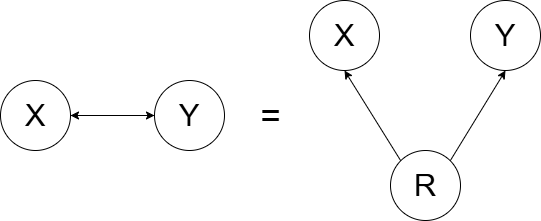
\includegraphics[width=0.5\textwidth]{rootification.png}
    \caption{String diagram of rootification}
    \label{fig:rootification}
\end{figure}
Through this transformation, the originally implicit confounding relationship is converted into an explicit latent variable, resulting in a causal structure with explicit latent parents. For instance: 

The second step constructs a \textbf{mechanism node} for each variable. 
For every endogenous variable $X$, the system creates a mechanism box $f_X$ representing the structural equation that determines $X$. 
The inputs of this mechanism box include all parent variables of $X$, together with an additional exogenous random variable $U_X$. 
These exogenous variables are provided by independent probability source nodes and represent the stochastic disturbances in the structural equations.

The third step establishes the \textbf{structural connections} between variables. 
Each directed edge $X \to Y$ in the causal graph is translated into a connection in the wiring diagram from the output of the mechanism $f_X$ to an input of the mechanism $f_Y$. 
In this way, the causal structure is fully encoded as a compositional diagrammatic representation.

This representation is consistent with the string-diagram semantics of causal models proposed by Lorenz and Tull \cite{intro_to_string_diagram}. In their framework, causal mechanisms can be interpreted as morphisms in a symmetric monoidal category, while causal graphs correspond to network diagrams formed by the composition of these morphisms. 
By compiling an ADMG into a wiring diagram, the causal model becomes a compositional diagrammatic structure, allowing reasoning to be carried out through diagram transformations.

The single-world causal diagram produced at this stage serves as the foundational structure for the subsequent algorithms. 
In the following steps, this diagram is further extended into a \textbf{parallel-world} graph structure in order to represent counterfactual queries. 

\section{Parallel-World Construction}
The second stage of the pipeline is parallel-world construction. This step lifts the single-world causal diagram into a multi-world representation in order to express counterfactual structure. This construction reflects the parallel-world semantics of counterfactual reasoning, where multiple hypothetical worlds are considered simultaneously under shared exogenous variables \cite{shpitser2007counterfactuals}.

Starting from the wiring diagram obtained via ADMG compilation, we construct multiple copies of the original causal model. Each copy corresponds to a different hypothetical intervention. These copies are then composed into a unified structure, referred to as the multiverse diagram. This diagram explicitly represents dependencies across different worlds. Each ``world'' corresponds to a specific interventional assignment. It is obtained via \textbf{diagrammatic surgery}, whereby all incoming edges to the intervened variables are removed and replaced by fixed inputs. From a categorical perspective, this operation is equivalent to replacing certain morphisms with constant morphisms, thereby altering the overall compositional structure of the diagram.

A key feature of the construction is the sharing of exogenous variables. Rather than duplicating noise sources independently across worlds, the same exogenous inputs are connected to all copies of the model. As a result, the different worlds remain \emph{coupled}. This coupling is essential, as counterfactual reasoning relies on comparing outcomes under different interventions while keeping the underlying randomness fixed. To formalise this process, we introduce two core concepts:
\begin{itemize}
\item \textbf{Sharp state:}
A sharp state deterministically assigns a variable to a fixed constant value. It is used to represent interventions, where a variable is no longer computed from its parents but instead fixed externally.

\item \textbf{Sharp effect:}
A sharp effect selects or constrains the value of a variable. It is used to represent observations or evidence.


\end{itemize}

Within the multiverse diagram, interventions are implemented by inserting sharp states, while observations can be expressed via sharp effects. Crucially, both are represented within the same diagrammatic language, providing a unified framework for intervention and conditioning.


Moreover, the resulting structure is inherently compositional. Each world provides a copy of the underlying mechanisms, while the shared exogenous variables ensure consistency across different worlds. Taken together, this construction encodes the counterfactual query within a single unified diagram. This corresponds precisely to the \textbf{parallel-world semantics} used in identification theory.

The third stage of the pipeline is \textbf{counterfactual simplification}, implemented by \texttt{simplify-cf}. Its purpose is to transform the multiverse diagram obtained from parallel-world construction into a more compact and semantically transparent representation.

The multiverse diagram is deliberately expanded during construction: in order to represent counterfactual objects under different interventional conditions, the causal mechanisms are replicated across multiple worlds, while shared exogenous variables couple these worlds together. This representation faithfully captures the counterfactual semantics, but may retain distinctions that are no longer necessary from a global perspective.

The role of \texttt{simplify-cf} is therefore to eliminate such redundant structure, while preserving the meaning of the query.

\section{Simplify-cf}
The third stage of the pipeline is \textbf{counterfactual simplification}, implemented by \texttt{simplify-cf}. This procedure is grounded in the theory of counterfactual identification developed in the causal inference literature, including the frameworks of Pearl and subsequent work by Shpitser and Pearl~\cite{pearl2009causality, shpitser2006identification}. In this work, these ideas are reinterpreted in a diagrammatic setting using string diagrams, following the categorical perspective of Lorenz and Tull~\cite{lorenz2023causal}. Its purpose is to transform the multiverse diagram obtained from parallel-world construction into a more compact and semantically transparent representation. The multiverse diagram is deliberately expanded during construction: in order to represent counterfactual objects under different interventional conditions, the causal mechanisms are replicated across multiple worlds, while shared exogenous variables couple these worlds together. This representation faithfully captures the counterfactual semantics, but may retain distinctions that are no longer necessary from a global perspective. The role of \texttt{simplify-cf} is therefore to eliminate such redundant structure, while preserving the meaning of the query.

The central idea of the algorithm is that duplication induced by world indices is only necessary when copies across different worlds correspond to genuinely distinct causal content. After the multiverse diagram is constructed, some nodes originating from different worlds may remain syntactically distinct while being semantically equivalent, in the sense that they represent the same counterfactual variable. This typically occurs in two cases. First, when the nodes correspond to the same endogenous variable and are evaluated under effectively identical interventional contexts. Second, when the differences between worlds do not influence the variable in question. In both situations, maintaining multiple copies reflects only a syntactic distinction rather than a semantic one. Therefore, such nodes should be identified and merged.

This merging operation can be understood both from a graph-theoretic and a categorical perspective. From the graph-theoretic viewpoint, it corresponds to a local contraction of the multiverse diagram. From the categorical viewpoint, it can be interpreted as imposing a quotient structure on the diagram, identifying semantically equivalent nodes as a single object.

Concretely, when multiple representatives across different worlds correspond to the same underlying variable, they are collapsed into a single representative, and the incident structure is redirected accordingly. The key point is not whether a colimit is constructed explicitly, but rather the guiding principle behind the operation: the resulting diagram should reflect the intrinsic counterfactual semantics, rather than the artefacts of duplication introduced during the multiverse construction.

A common source of equivalence arises when certain variables are unaffected by the interventions that distinguish different worlds. If a variable in two worlds is governed by the same structural mechanism and depends on the same upstream exogenous inputs, then the corresponding copies compute the same quantity and should therefore be identified. In addition, interventions themselves also induce further simplifications. In the graphical representation, an intervention replaces the original mechanism of a variable with a fixed input, which naturally corresponds to a \textbf{sharp state} in the categorical language. Once a variable is fixed, this information can propagate downstream through the diagram. Subsequent mechanisms no longer treat this input as a free variable, but instead as a constant. Then, nodes that were previously distinct may become equivalent once this fixed value is taken into account. The treatment of observational conditions is analogous. When the query includes evidence, such constraints can be represented using a \textbf{sharp effect}, whose role is to restrict the admissible values of a variable. This restriction eliminates those worlds or branches that are incompatible with the given condition, thereby reducing the portion of the diagram that must be retained. In other words, both interventions and observations drive the diagram towards a more canonical form: sharp states fix values, while sharp effects eliminate branches that do not satisfy the imposed conditions.

In addition to merging equivalent nodes, \textbf{simplify-cf} also removes worlds or subgraphs that no longer contribute to the target expression. After node identification and constraint propagation, certain parts of the multiverse diagram may become disconnected from the query variable, or contain information that has already been fully absorbed elsewhere. Such components are therefore redundant and can be safely eliminated without affecting the semantics of the query.

A counterfactual query may admit multiple syntactic representations, which do not necessarily yield identical multiverse diagrams after the initial expansion. However, after simplification, these representations should converge to the same, or essentially equivalent, diagrammatic form. This canonicalisation ensures that the resulting representation does not depend on the particular syntactic form of the original query, but instead reflects its underlying semantics. In turn, simplify-cf not only provides a more stable and well-defined input for subsequent identification algorithms, but also significantly reduce computational cost for the whole algorithm.

We now describe the simplify-cf procedure explicitly as a sequence of local rewriting steps applied to the multiverse diagram.

\paragraph{Step 1: Eliminating discard.}
The first step removes all discard nodes from the diagram. 
In the diagrammatic semantics, a discard represents marginalisation over a variable that does not appear in the final query. By repeatedly exploiting the defining properties of channels together with the interaction laws of copy maps, discard operations can be pushed downward through the diagram. Whenever a discard reaches a copy node, the corresponding discarded branch can be removed directly. This process is applied iteratively until no discard nodes remain in the diagram. 

\paragraph{Step 2: Separating sharp effects.}
The second step handles observational constraints represented by \emph{sharp effects}. When a sharp effect is connected to multiple branches through a copy map, apply the equality given in (\ref{fig:‘separate’}) to separate it from the shared structure. The purpose of this transformation is to disentangle observational conditions that are initially coupled within the same copying structure. By doing so, each constraint becomes localised and can be propagated 
and simplified independently in subsequent steps. 

\begin{figure}[H]
    \centering
    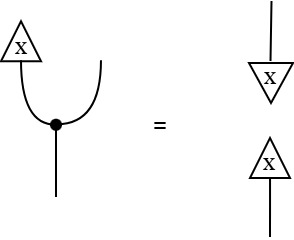
\includegraphics[height=0.2\textwidth]{sharp.jpg}
    \caption{‘separate’}
    \label{fig:‘separate’}
\end{figure}

\paragraph{Step 3: Iterative simplification along a variable order.}
After eliminating discard nodes and separating shared sharp effects, the algorithm processes variables in a topological order $\pi$, starting from lower-level root nodes. The reason for adopting this order is that simplifications at lower-level variables may change the input form of higher-level mechanisms, thereby creating conditions for further merging and rewriting.

In Step 3.1, if several instances of $f_L$ have identical inputs, then these copies represent the same deterministic computation and can therefore be identified as the same object, and replaced by a single instance of $f_L$ in the diagram. This eliminates redundancies that are introduced solely by world duplication but have no semantic difference.

In Step 3.2, after merging these equivalent mechanisms, it may happen that a sharp effect is connected via a copy map to the output of some $f_L$. In this case, the diagram needs to be further rewritten follow the graph(\ref{fig:‘step 3.2’}) so that these observational constraints can be propagated backwards and appropriately separated onto more local input branches.
\begin{figure}[H]
    \centering
    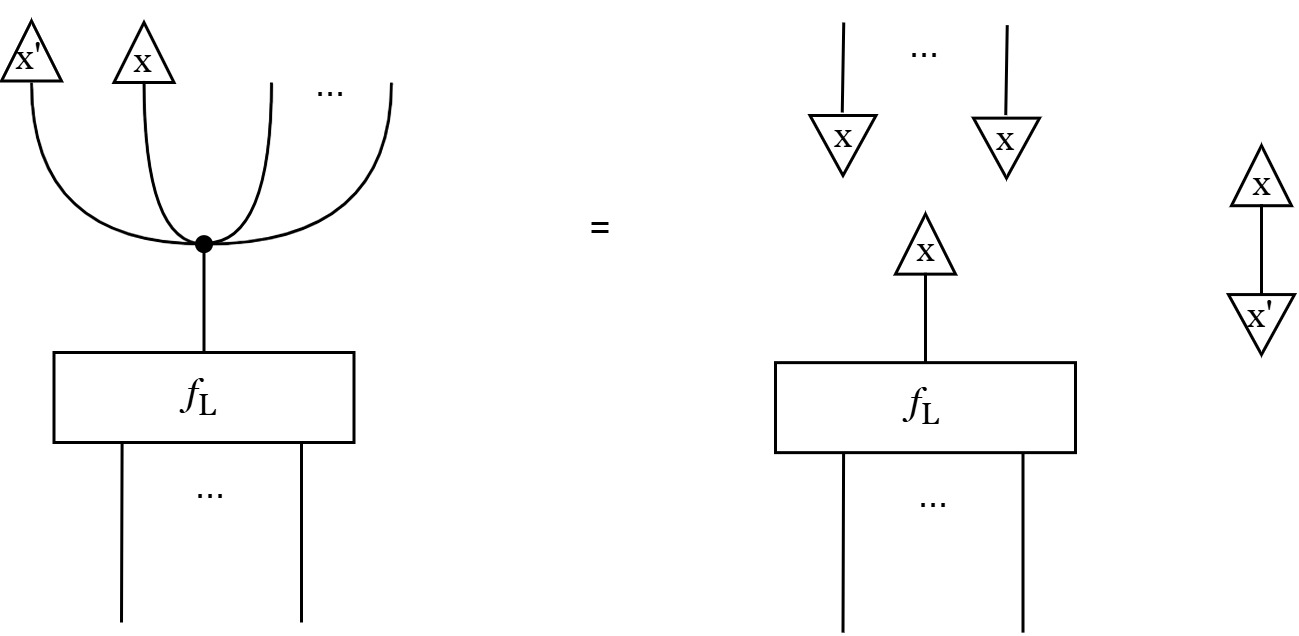
\includegraphics[height=0.3\textwidth]{3.2.jpg}
    \caption{Step 3.2}
    \label{fig:‘step 3.2’}
\end{figure}

The algorithm repeats the above checks along the given variable order until no further simplifications according to Step 3.1 or Step 3.2 can be applied. At this point, the diagram is in normal form with respect to this set of rewriting rules.

\paragraph{Step 4: Replacing isolated mechanisms with constants.}
When Step 3 can no longer be applied, the algorithm finally checks whether there exists a mechanism $f_X$ that takes only its noise state $\lambda_X$ as input and is no longer shared, via copy maps, with instances in other worlds. In this case, the mechanism no longer participates in any substantial way in the interactions of the multiverse structure, and therefore $\lambda_X$ together with $f_X$ can be replaced by the corresponding constant node $c_X$. This step further compresses substructures that have become fully localised. 

Finally, the algorithm outputs the simplified diagram and uses it as the input for subsequent 
identifiability analysis.

\paragraph{Example.}
We consider a causal model motivated by a daily commuting scenario. Let 
$O = \{W, T, M, L, Y\}$ denote the set of variables, where $W$ represents 
weather, $T$ departure time, $M$ mode of transport, $L$ lateness, and $Y$ 
the final work performance.

The causal structure is given by the directed edges
\[
W \to T, \quad W \to M, \quad T \to L, \quad M \to L, \quad L \to Y,
\]
together with a bidirected edge
\[
T \leftrightarrow Y,
\]
representing latent confounding between departure time and the final outcome.

Suppose the observational distribution $P^*(O)$ is given. We consider the 
following counterfactual query:
\[
P^s_{M_3}\!\bigl(
Y(1)\mid W(2)=w,\; T(2)=t',\; M(3)=m
\bigr),
\qquad
s=\{do(T(1)=t),\; do(W(3)=w)\}.
\]

This query involves three distinct worlds. In the first world, we intervene on the departure time by setting $T$ to $t$, and evaluate the resulting outcome $Y(1)$. The second world corresponds to the factual setting, where the weather is observed to be $w$ and the individual departs at time $t'$. The third world encodes an auxiliary intervention $do(W=w)$, under which the mode of transport is observed to be $M(3)=m$.

Intuitively, this query can be understood as follows: for an individual who, on a given day with weather condition $w$, actually departs at time $t'$, what would their work performance $Y$ have been had they instead departed at time $t$? At the same time, we incorporate additional information that under the same weather condition $w$, the individual would choose transport mode $m$. This auxiliary information helps constrain the individual's behaviour across different interventional scenarios. The identification problem is to determine whether this counterfactual quantity can be uniquely expressed in terms of the observational 
distribution $P^*(O)$.

Begin with the ADMG representation, which contains bidirected edges to represent latent confounding. However, this representation presents a limitation: the latent variables are implicit, making it difficult to directly express counterfactual operations on the graph. To address this issue, we perform \textbf{rootification}, replacing each bidirected edge with an explicit exogenous variable (\ref{fig:(a)}. In this way, latent confounding is made explicit. As a result, each variable is now computed by a structural mechanism, and the graph becomes a standard causal generative model. Next, we compile this causal model into a \textbf{string diagram} (\ref{fig:(b)}) and the corresponding FCM is \ref{fig:(c)}. In this representation, each variable corresponds to a mechanism box, whose inputs are its parent variables and exogenous variables, and whose output is the variable itself. This representation is compositional, allowing subsequent transformations to be expressed via local rewriting rules. To represent counterfactual queries, we introduce a \textbf{parallel-world structure}. Concretely, we replicate the single-world model and apply different interventions to different copies (\ref{fig:multi})(note that The blue dashed box represents normalization). Crucially, these worlds are not independent; instead, they are coupled through shared exogenous variables, ensuring that they correspond to the same underlying unit.

\begin{figure}[t]
\centering

\subfloat[ADMG\label{fig:(a)}]{%
    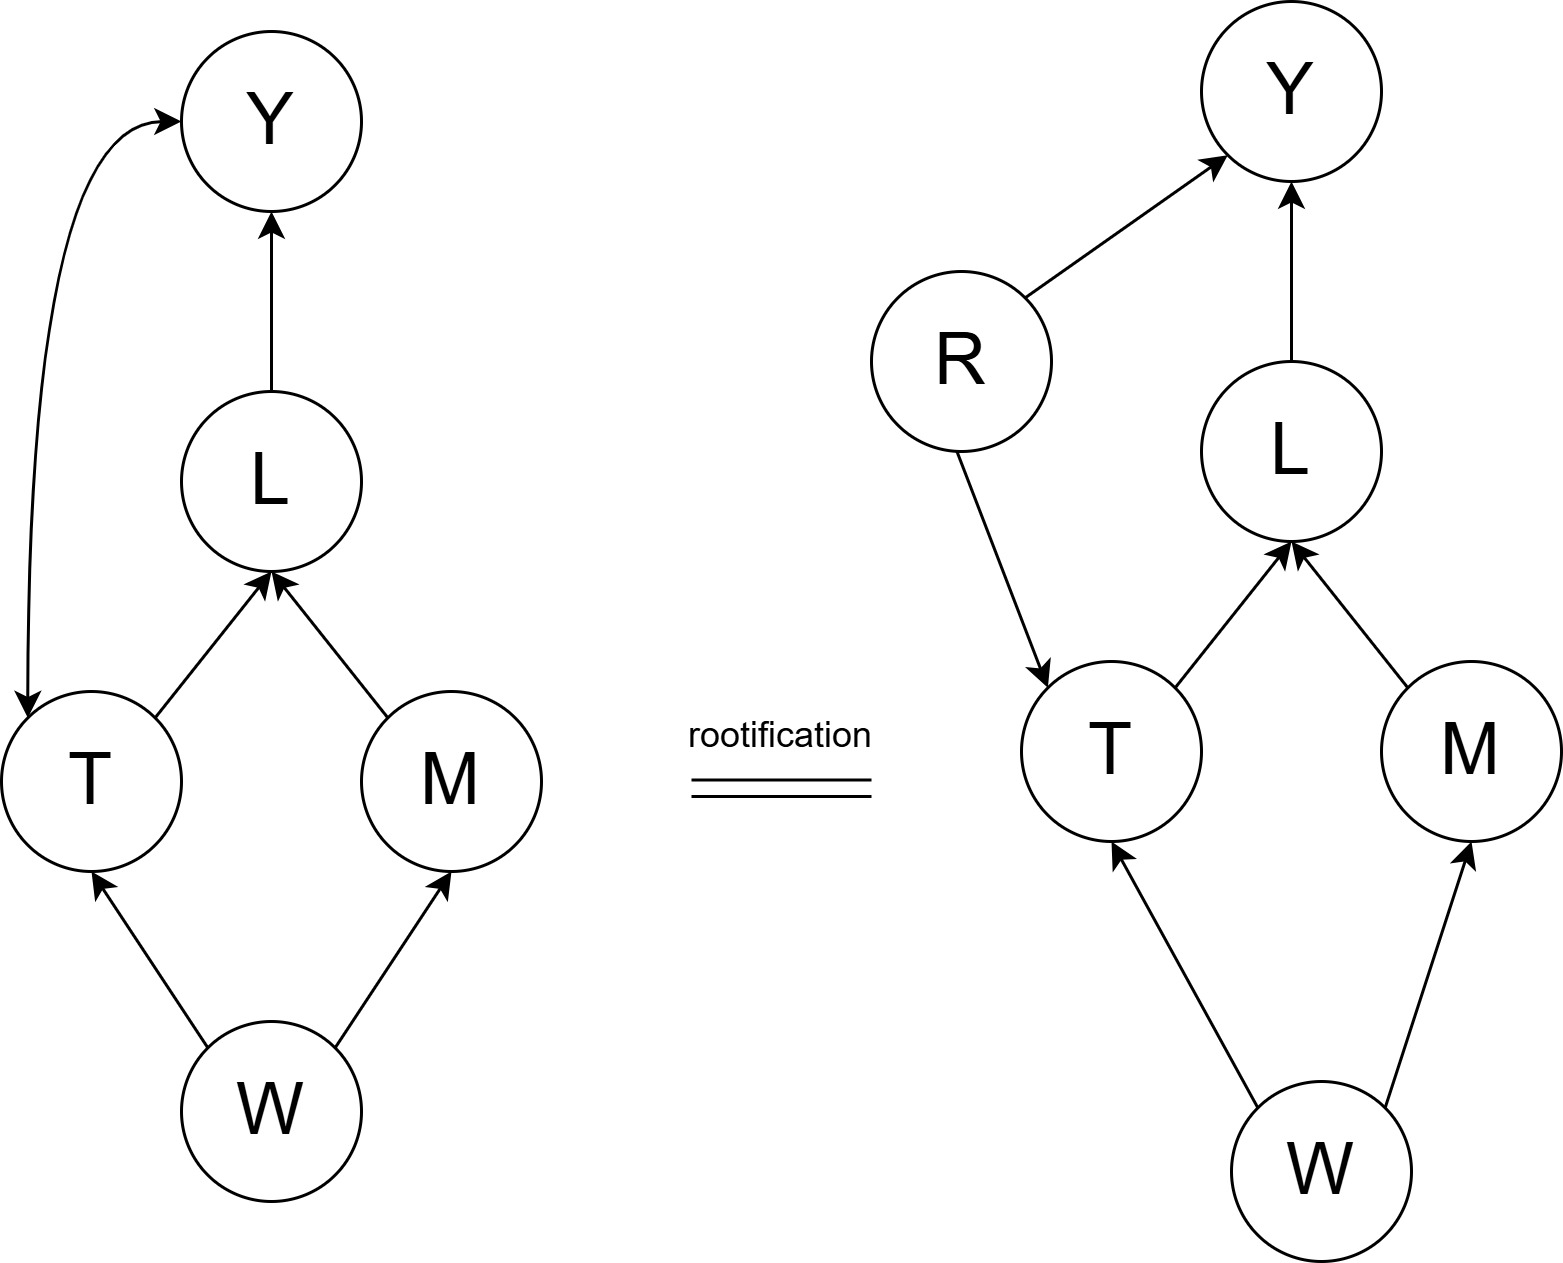
\includegraphics[width=0.4\textwidth]{ADMG.jpg}
}
\hfill
\subfloat[String\label{fig:(b)}]{%
    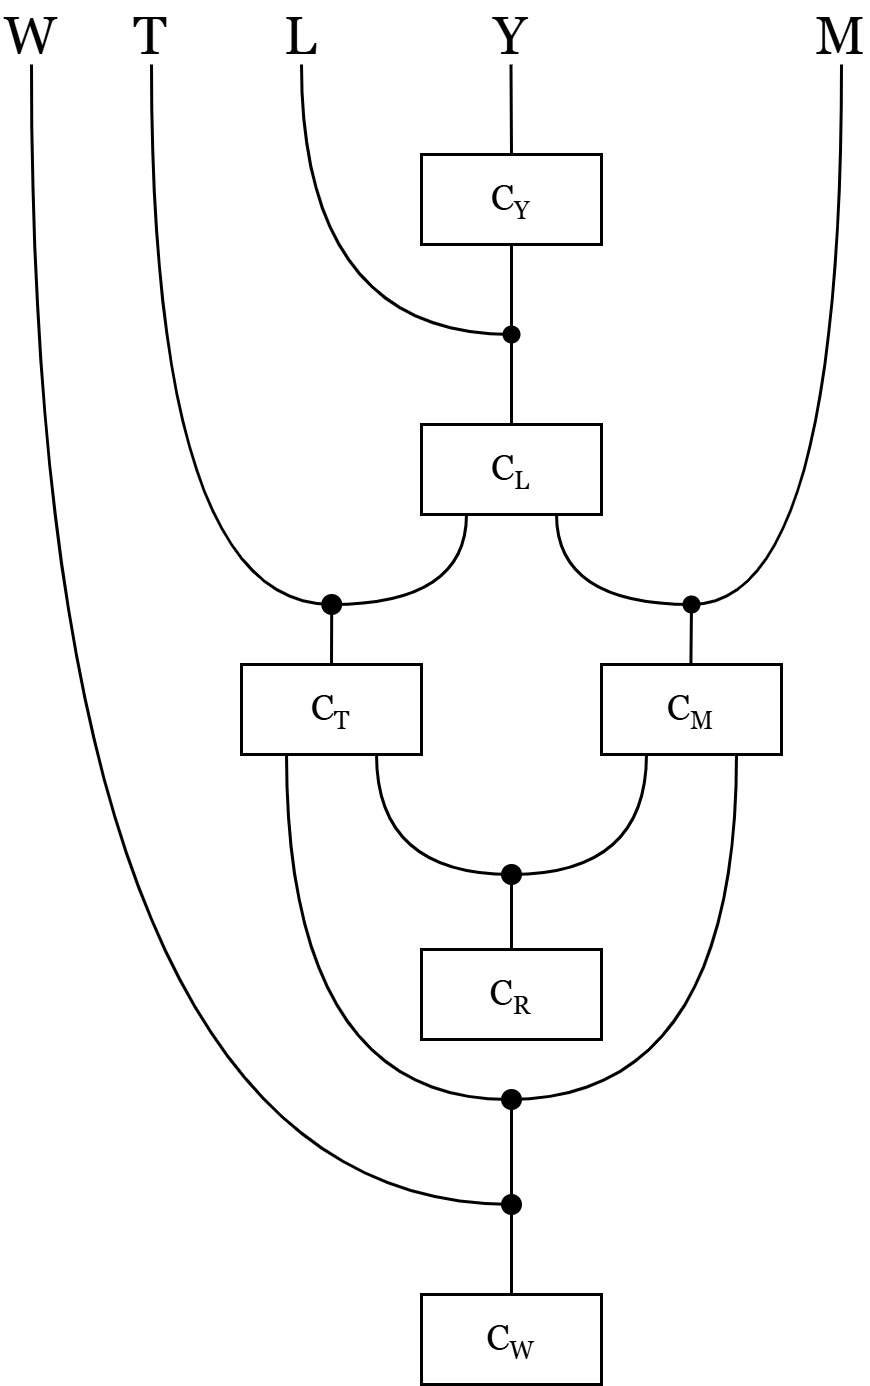
\includegraphics[width=0.23\textwidth]{Stringdiagram.jpg}
}
\hfill
\subfloat[FCM\label{fig:(c)}]{%
    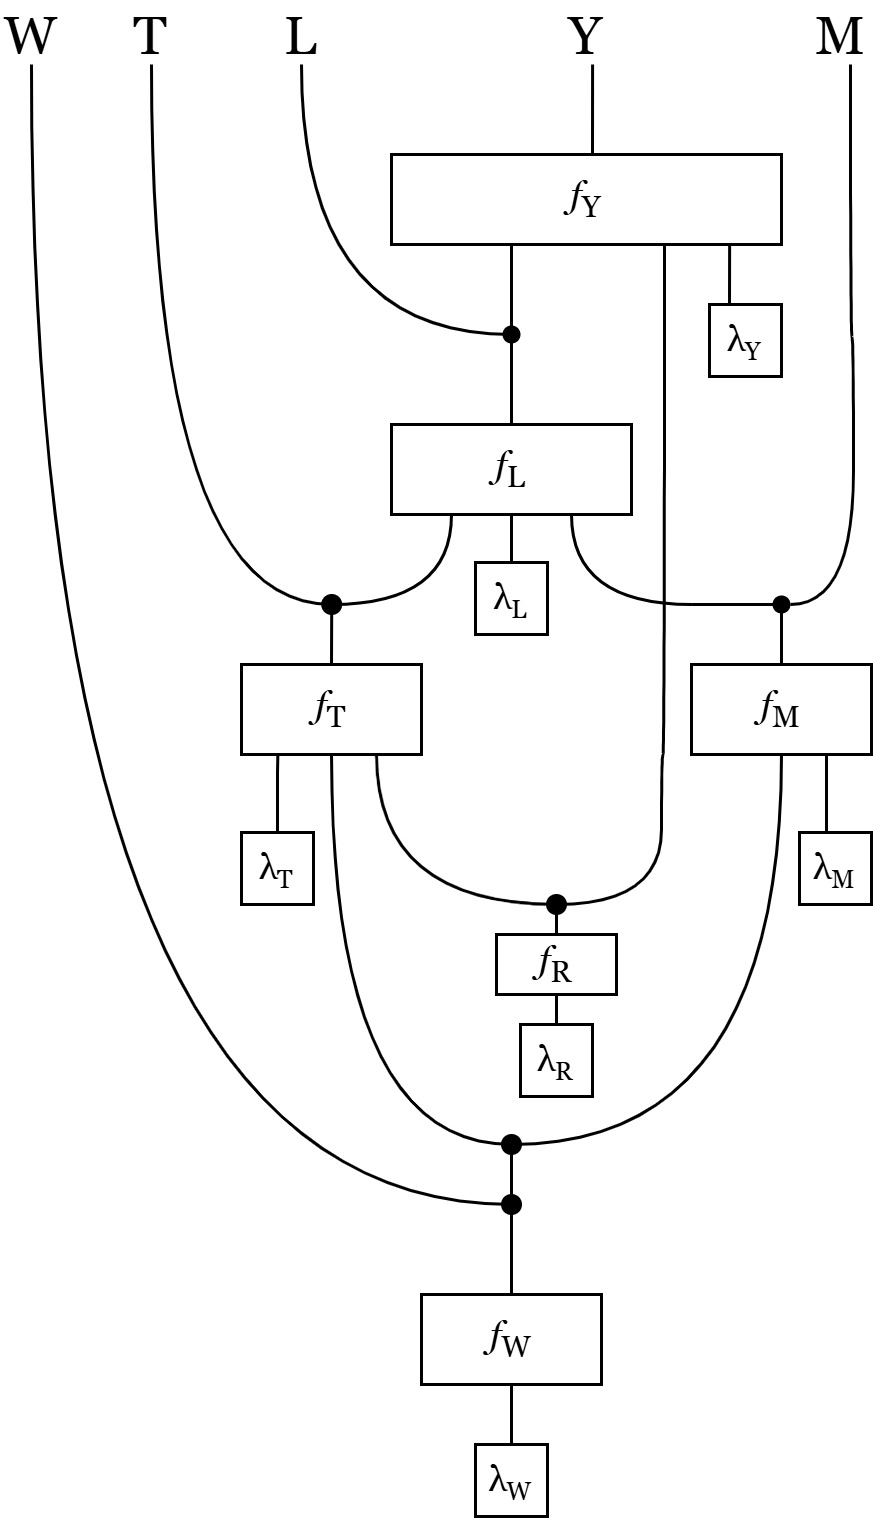
\includegraphics[width=0.23\textwidth]{FCM .jpg}
}
\label{fig:pipeline}
\end{figure}

\begin{figure}[H]
    \centering
    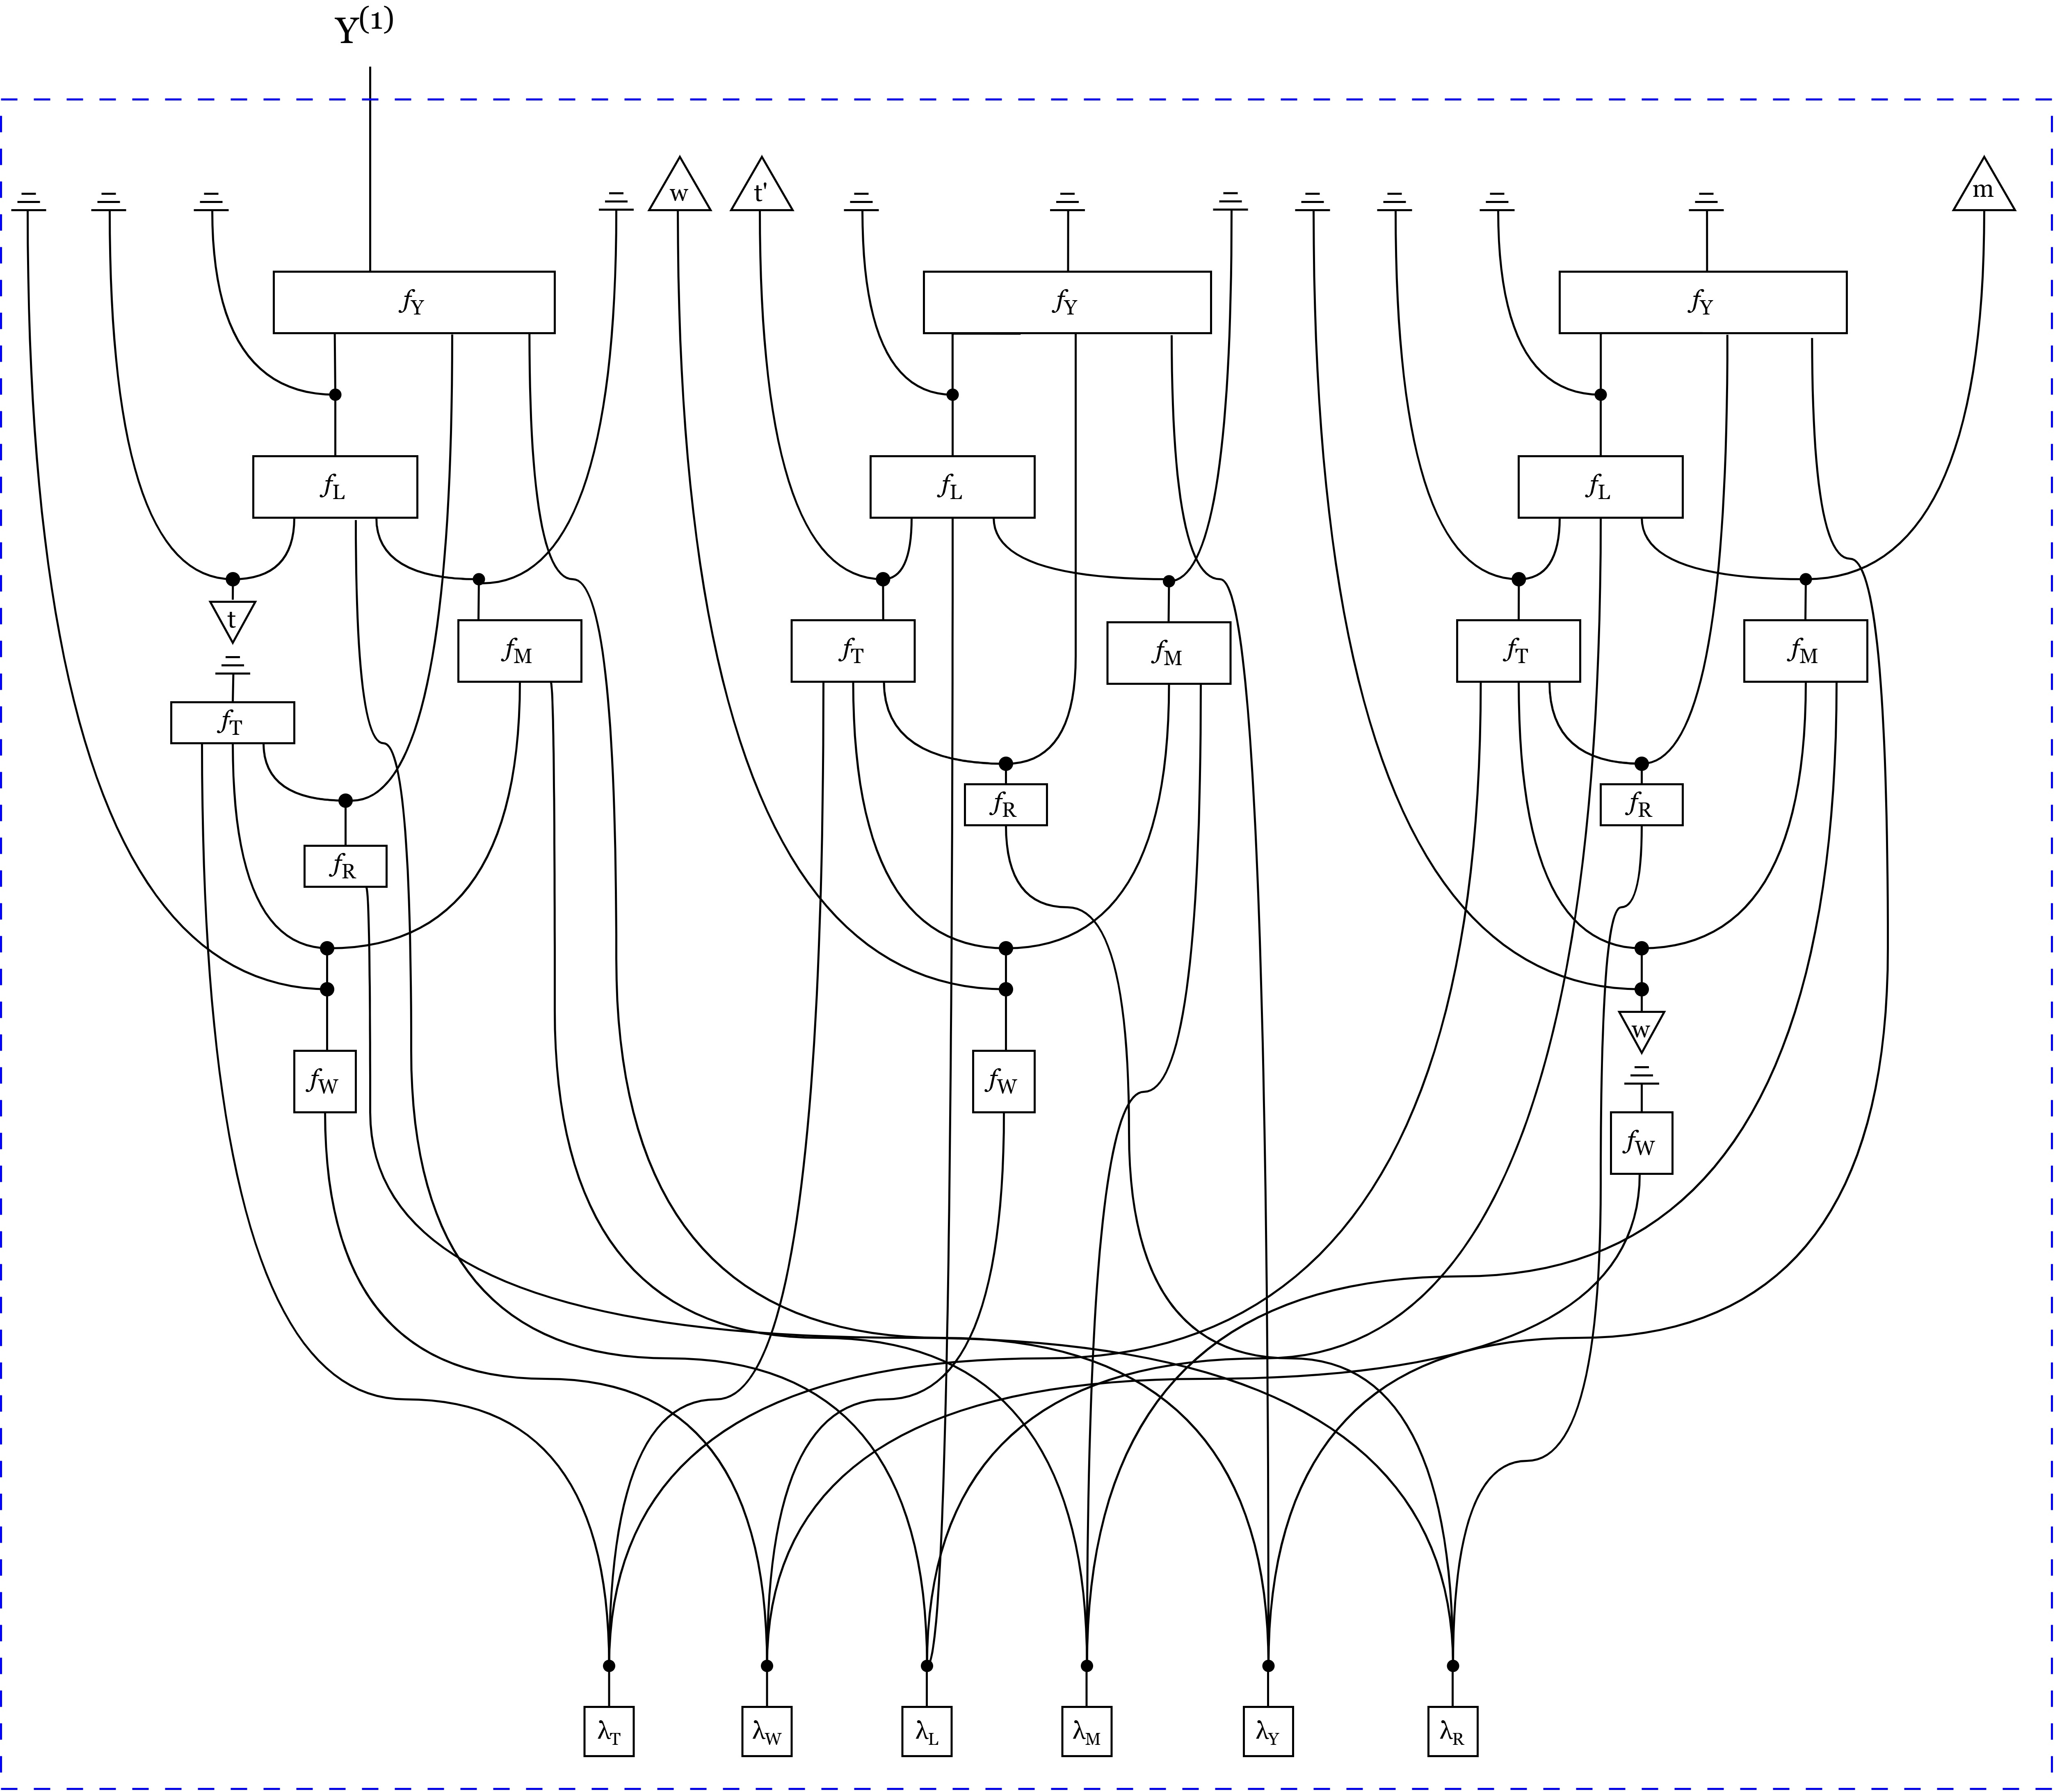
\includegraphics[height=0.6\textwidth]{multi.jpg}
    \caption{multiverse}
    \label{fig:multi}
\end{figure}
At this point, all preparatory steps for \textbf{simplify-cf} have been completed, and we proceed to the simplification stage. \ref{fig:simplify} illustrates how the multiverse diagram is progressively reduced under successive rewriting steps. The first diagram shows the result after Step~1 (dropping discard branches): all branches that only lead to discard and do not contribute to the query \(Y^{(1)}\) or the observational constraints are removed. The resulting diagram retains only the relevant structure, but still contains redundancies introduced by world duplication.

\((a)\) corresponds to Step~2, where sharp effects are separated. Observational constraints are detached from shared copy structures and relocated into more local positions, enabling them to be propagated independently in later steps.

\((b)\) corresponds to Step~3.1, where equivalent mechanisms are merged. Mechanism copies with identical inputs are identified as the same computation and replaced by a single instance, eliminating redundancies caused by world duplication.

\((c)\) corresponds to Step~3.2, where sharp effects are propagated. Observational constraints are pushed backward through mechanisms and further localised, allowing certain substructures to be separated from the main diagram.

\((d)\) corresponds to another application of Step~3.1. After constraint propagation, new equivalences emerge, enabling further merging of mechanisms and additional compression of the diagram.

\((e)\) corresponds to another application of Step~3.2, where constraints associated with \(M\) are fully separated into independent subgraphs, leaving only the core structure relevant to the target variable in the main diagram.

Finally, \((f)\) corresponds to Step~4, where isolated mechanisms are replaced by constants. Mechanisms that depend only on their local noise and no longer participate in cross-world interactions are collapsed into constant nodes, yielding the final normal form of the diagram.


\begin{figure}[H]
    \centering
    \includegraphics[width=1.05\textwidth]{simplify.jpg}
    \caption{simplify}
    \label{fig:simplify}
\end{figure}


\section{ID-CF}
Given the simplified diagram produced by \textbf{simplify-cf}, the final stage of the pipeline is to determine whether the counterfactual query is \textbf{identifiable}, and, if so, to construct an equivalent probabilistic expression. This task is carried out by the \textbf{ID-CF algorithm}. The algorithm extends the classical identification procedures of Shpitser and Pearl to the diagrammatic setting. While \textbf{simplify-cf} reduces the diagram to a canonical form, ID-CF operates on this structure to determine whether it can be rewritten entirely in terms of distributions in $P^*$. The central idea of the ID-CF algorithm is to analyse the structure of the simplified diagram and decompose it into smaller components that can be treated independently, thereby determining identifiability. However, unlike traditional graph-based approaches, this decomposition is performed directly on the diagrammatic representation (i.e., wiring diagrams). This requires identifying substructures that correspond to regions of the underlying causal graph affected by latent confounding. 

To formalise this decomposition, we introduce the notion of an \textbf{R-fragment}.

\paragraph{R-fragments.}

\textbf{Definition.}
An \emph{R-fragment} is a maximal connected subdiagram of the simplified counterfactual diagram $D'$ satisfying the following conditions:

\begin{enumerate}
    \item The fragment contains a set of endogenous variables $X \subseteq O$, together with their associated mechanisms $c_X$ and any incident copy maps.

    \item For any two variables $X, Y$ in the fragment, there exists a path between them consisting only of:
    \begin{itemize}
        \item bidirected connections induced by shared root nodes (i.e. latent confounding), and
        \item copy-map connections that preserve dependence on the same exogenous inputs.
    \end{itemize}

    \item The fragment is maximal with respect to this property, i.e. no additional variable can be included without violating the above connectivity condition.
\end{enumerate}

Equivalently, an R-fragment corresponds to a maximal set of variables whose associated mechanisms remain coupled through shared latent variables after the application of \textbf{simplify-cf}. In this sense, R-fragments provide the diagrammatic counterpart of \emph{c-components} (also known as districts) in ADMGs.

The role of R-fragments in the ID-CF algorithm is to define the minimal units on which identification must be performed. Since the variables within the same R-fragment are coupled through latent confounding, they cannot be decomposed into independent components. Therefore, identification must be carried out jointly over the entire fragment.

We now proceed to describe the detailed procedure of the ID-CF algorithm. 

\paragraph{Step 1: Checking noise absorption.}  

Before proceeding, the algorithm verifies that all noise variables have been absorbed during simplify-cf.   If there exists a variable $X$ such that its noise state $\lambda_X$ remains explicitly in the diagram, this indicates that the corresponding latent dependency cannot be eliminated. In this case, the counterfactual query is not identifiable, and the algorithm returns \textbf{FAIL}.

\paragraph{Step 2: Decomposition into R-fragments.}  The simplified diagram is partitioned into a collection of R-fragments. Each fragment corresponds to a maximal confounded component, and can be treated as a candidate unit for identification.  This decomposition isolates the parts of the diagram that must be analysed jointly due to shared latent structure.

\paragraph{Step 3: Iterative checking and rewriting}

For each R-fragment $F_l$, the algorithm examines all occurrences of each variable $X \in O$ that appear as the type of wires within the fragment. The goal is to determine whether these occurrences admit a \emph{consistent assignment}, which is a necessary condition for rewriting the fragment in terms of $P^*$.

This check is performed by distinguishing two cases, depending on whether the mechanism $c_X$ appears inside the fragment.

\medskip

\textbf{Case 1: $c_X \in F_l$.}

In this case, the fragment contains the mechanism that generates $X$, and therefore the value of $X$ is determined internally within the fragment.

\begin{itemize}
    \item If the output of $c_X$ is not composed with any sharp effect, and no additional wires of type $X$ appear in $F_l$, then no consistency constraint is imposed, and no action is required.
    
    \item If the output of $c_X$ is composed with a sharp effect fixing $X = x$, then all other occurrences of $X$ within the fragment must also take the same value $x$. This includes occurrences arising from copy maps or downstream dependencies.
    
    \item If all occurrences of $X$ agree on the same value $x$, the diagram can be rewritten by merging these occurrences into a single representative(\ref{fig:case1}).
    \begin{figure}[H]
        \centering
        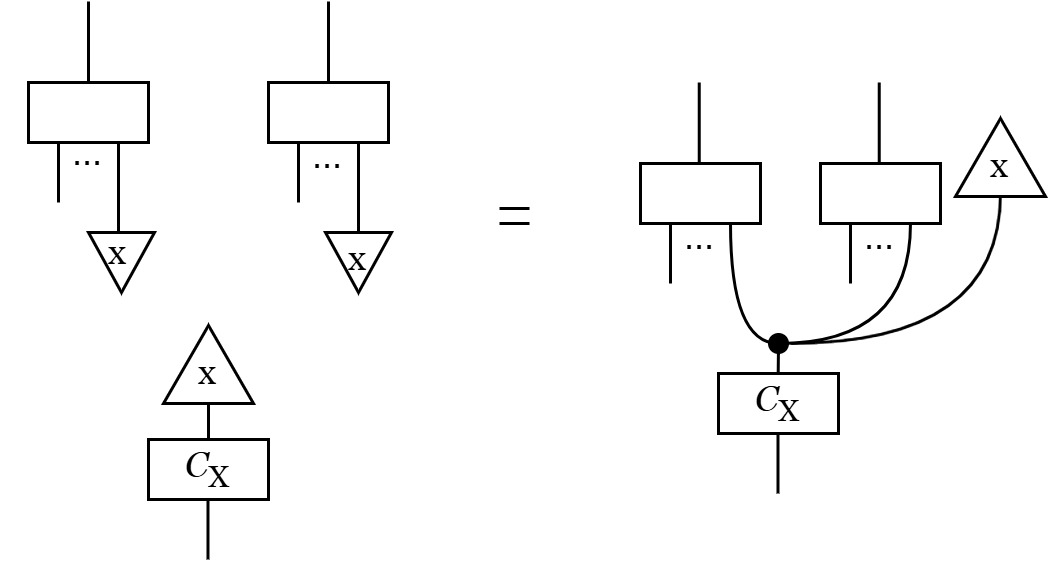
\includegraphics[height=0.3\textwidth]{idcfcase1.jpg}
        \caption{case1}
        \label{fig:case1}
    \end{figure}    
    
    
    \item Otherwise, if different occurrences of $X$ are assigned incompatible values, the fragment contains an intrinsic inconsistency, and the algorithm returns \textbf{FAIL}.
\end{itemize}

\medskip

\textbf{Case 2: $c_X \notin F_l$.}

In this case, the fragment does not contain the mechanism generating $X$, and all occurrences of $X$ must originate externally.

\begin{itemize}
    \item If all input wires of type $X$ in $F_l$ are obtained via copy maps from the same output of $c_X$ in another fragment, then they are already consistent by construction, and no further action is required.
    
    \item If the inputs are fixed by sharp states to a common value $x$, then all occurrences can be merged into a single constant representative(\ref{fig:case2}).
    
    \begin{figure}[H]
        \centering
        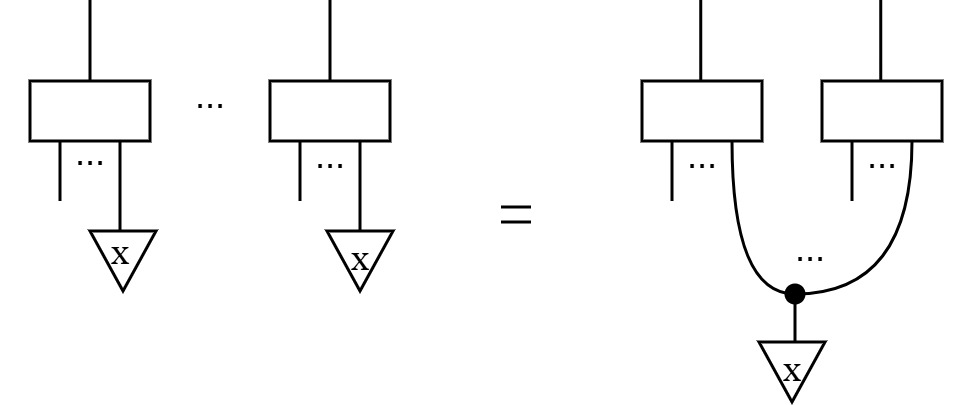
\includegraphics[height=0.3\textwidth]{idcfcase2.jpg}
        \caption{case2}
        \label{fig:case2}
    \end{figure} 
    
    \item Otherwise, if the fragment contains multiple occurrences of $X$ that originate from different sources or are assigned different values, then no consistent assignment exists, and the algorithm returns \textbf{FAIL}.
\end{itemize}

\medskip

Intuitively, this step ensures that each R-fragment admits a well-defined interpretation as a single probabilistic unit. Variables within the fragment must behave as if they are consistently instantiated across all occurrences. If this condition is violated, the fragment cannot be expressed as an interventional distribution, and the counterfactual query is not identifiable.

\paragraph{Step 4: Fragment rewriting.} Once consistency has been established, each R-fragment is rewritten as an interventional distribution. Concretely, each fragment is replaced by a term of the form \[ P(C_l, F_l^{out} \mid do(D_l), do(F_l^{in}))\] as shown in (\ref{fig:idcf3}).
\begin{figure}[H]
    \centering
    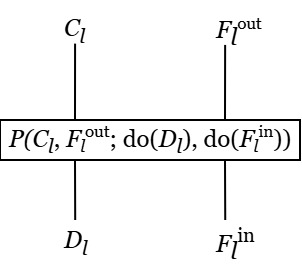
\includegraphics[height=0.3\textwidth]{idcf3.jpg}
    \caption{idcf3}
    \label{fig:idcf3}
\end{figure} 

\paragraph{Step 5: Composition and normalisation.}
After all fragments have been processed, the resulting expressions are composed according to the structure of the diagram. The final result is then normalised to obtain the desired counterfactual expression. 

We now return to the running example to illustrate how the ID-CF algorithm operates on the simplified diagram.

First, recall that after applying \texttt{simplify-cf}, all noise variables $\lambda_X$ have been absorbed into their corresponding mechanisms $c_X$. Therefore, the condition checked in Step 1 is satisfied, and the algorithm does not terminate with failure at this stage.

Next, in Step 2, the diagram is decomposed into a collection of R-fragments. As shown in \ref{fig:R-fragment}, the simplified diagram can be partitioned into several disjoint subdiagrams according to the confounded structure of the underlying graph. These fragments are indicated by dashed boundaries, each representing a maximal set of variables that remain coupled through shared latent dependencies. This decomposition isolates the components that must be analysed jointly in the subsequent steps.
\begin{figure}[H]
    \centering
    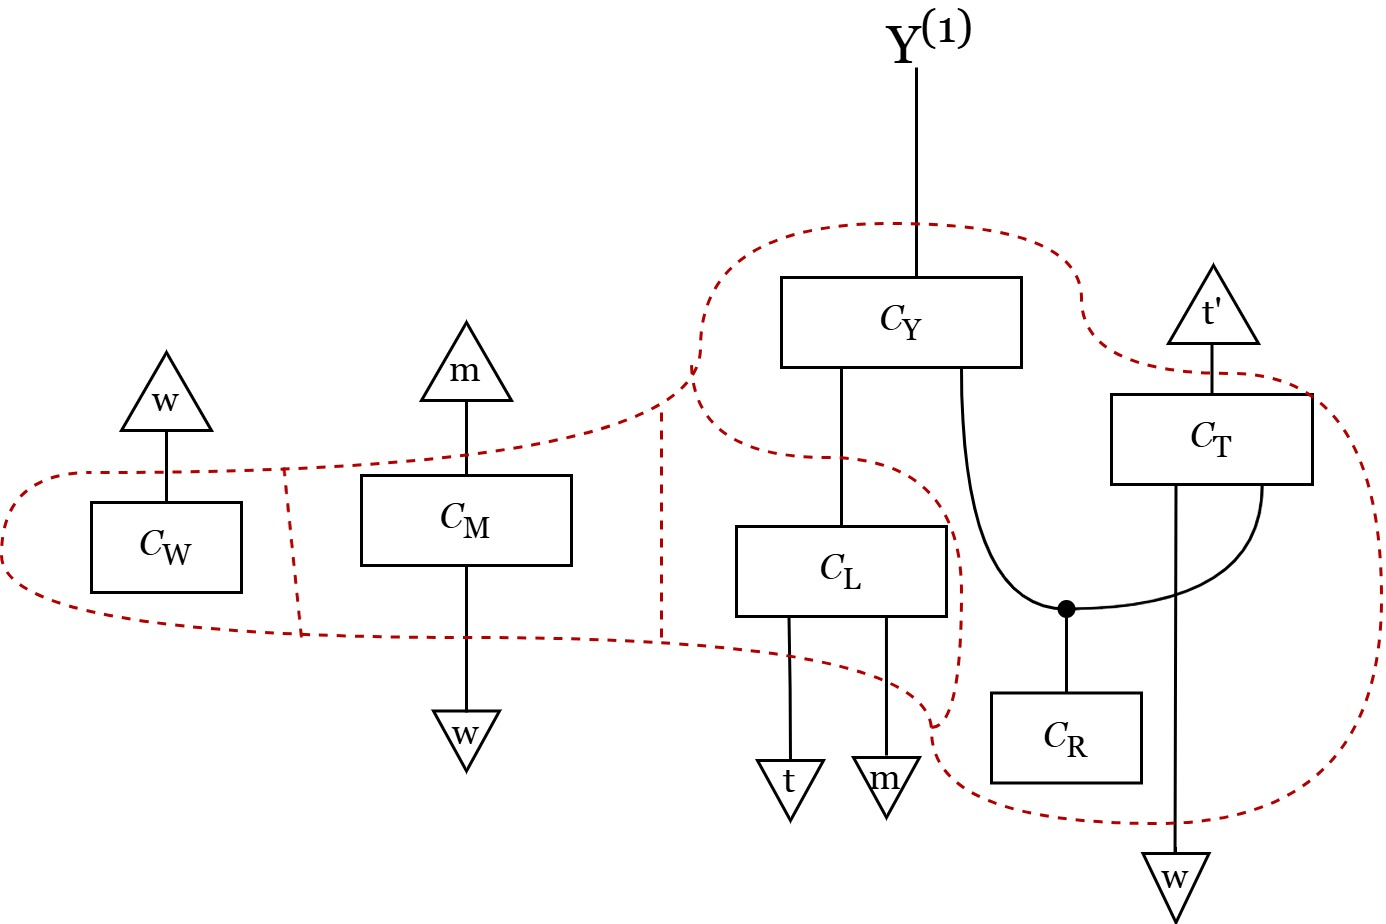
\includegraphics[height=0.4\textwidth]{R-fragment.jpg}
    \caption{R-fragment}
    \label{fig:R-fragment}
\end{figure} 

We then proceed to the recursive stage of the algorithm. In Step 3, the algorithm performs consistency checking within each R-fragment. For each fragment, all occurrences of each variable are examined to determine whether they admit a consistent assignment. In this example, the values imposed by interventions and observations are propagated through the diagram via copy maps, and no conflicting assignments arise. As a result, all fragments satisfy the consistency condition, and no failure is triggered.

Having established consistency, Step 4 rewrites each R-fragment as an interventional distribution. As shown in \ref{fig:idcf4}, each fragment is replaced by a probabilistic expression that depends only on its inputs, outputs, and the corresponding interventions. This transformation converts the diagrammatic representation into a collection of interventional terms expressed in $P^*$.
\begin{figure}[H]
    \centering
    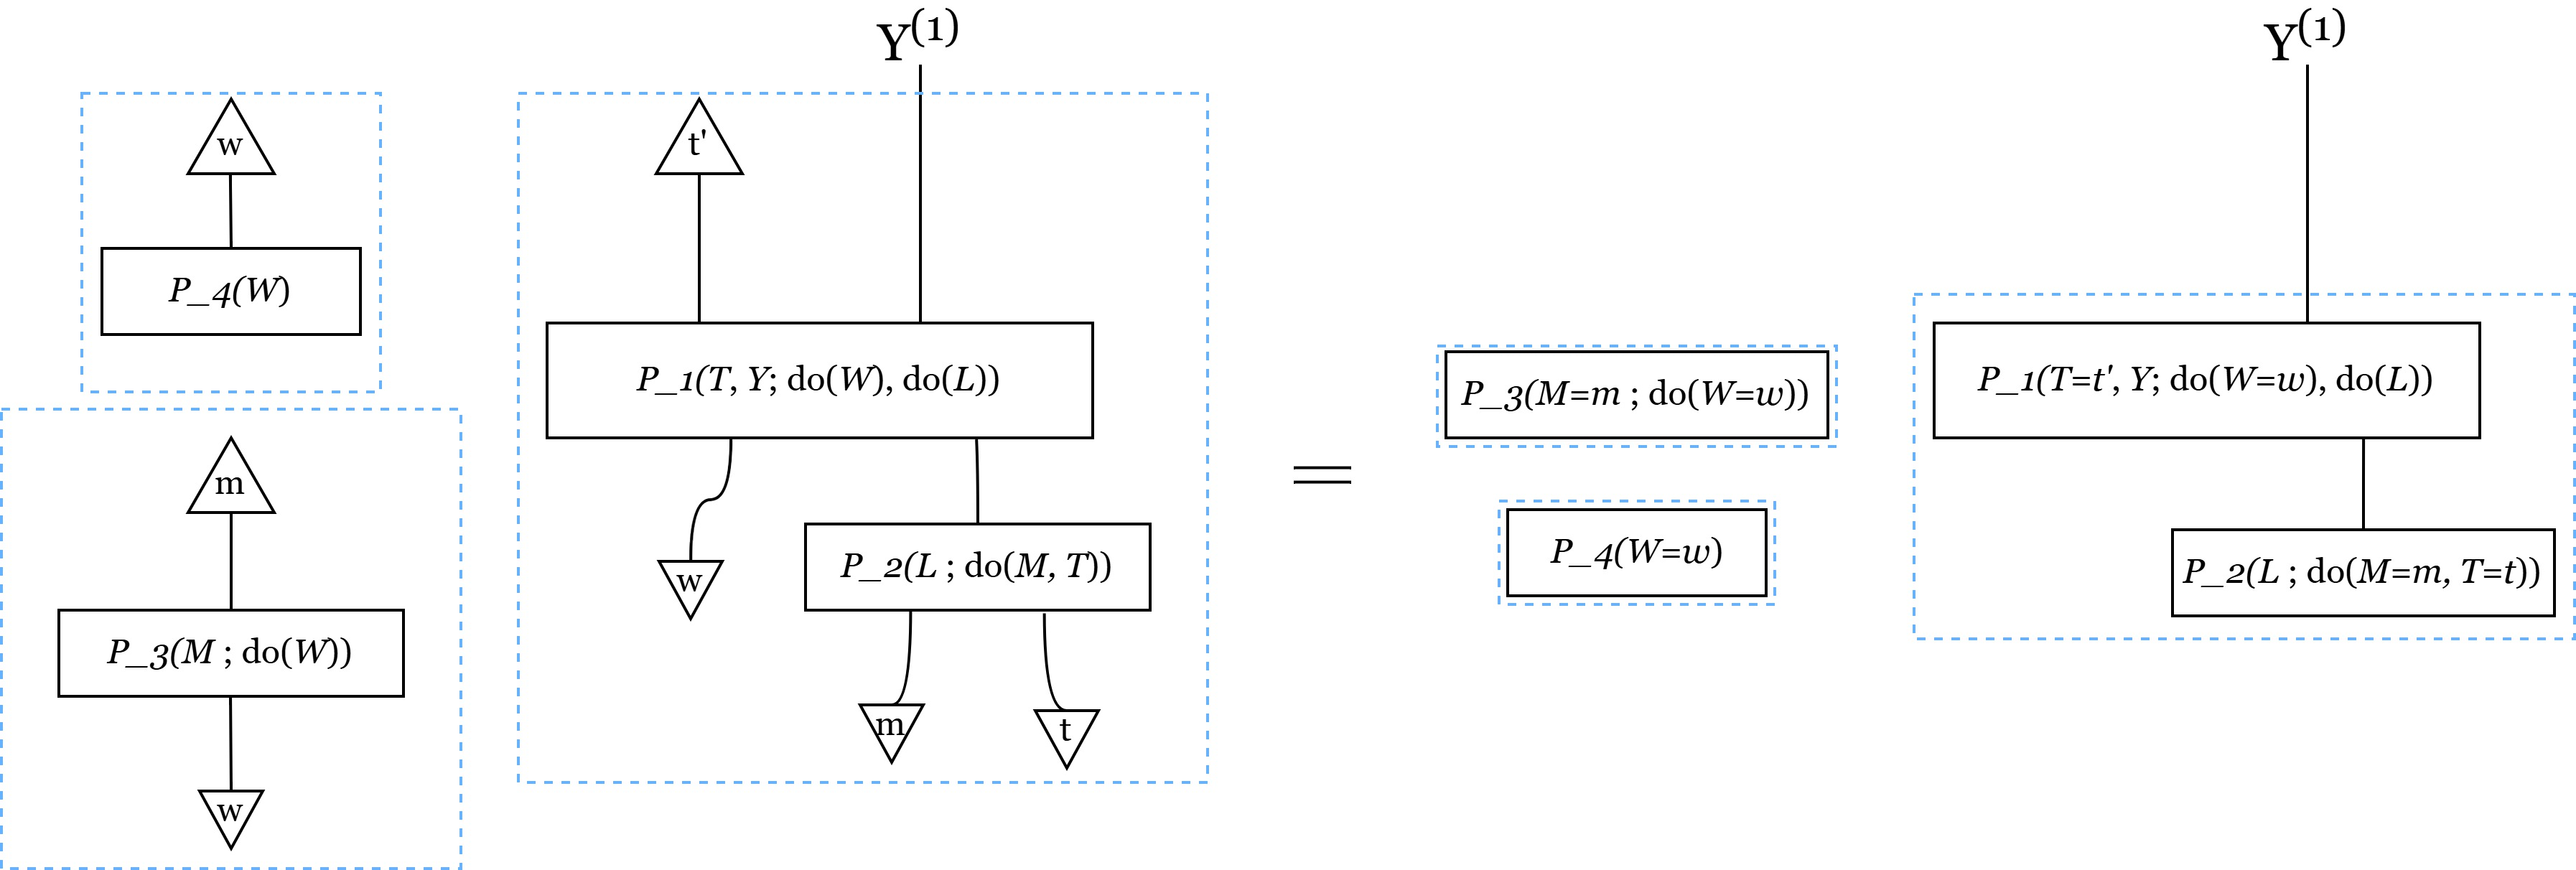
\includegraphics[height=0.4\textwidth]{idcf4.jpg}
    \caption{idcf4}
    \label{fig:idcf4}
\end{figure} 


Finally, these expressions are composed according to the structure of the diagram, and the resulting expression is normalised to obtain the final counterfactual quantity. This yields the desired identifiable expression.

\chapter{Implementation}

\section{ADMG Compilation}
The implementation begins by compiling an input acyclic directed mixed graph (ADMG) into a diagrammatic structural causal model represented as a \texttt{Catlab} wiring diagram. 
This compilation stage consists of two main steps: first, bidirected edges are transformed into explicit latent roots; second, the resulting confounded graph is translated into a network of mechanism and exogenous-noise boxes.

Two graph-level data structures are used in the implementation. 
An \texttt{ADMGModel} stores the observed directed edges and bidirected edges separately:
\[
\texttt{directed} : \texttt{Vector\{Pair\{Symbol,Symbol\}\}}, \qquad
\texttt{bidirected} : \texttt{Vector\{Pair\{Symbol,Symbol\}\}}.
\]
After latent expansion, the graph is represented as a \texttt{ConfoundedModel}, consisting of the directed edges together with a dictionary mapping each latent root to the variables it confounds:
\[
\texttt{latents} : \texttt{Dict\{Symbol, Vector\{Symbol\}\}}.
\]
This separation makes the preprocessing stage explicit: the ADMG is treated as the input format, while the confounded model is the internal representation used for diagram construction.

The function \texttt{rootify(model::ADMGModel)} converts each bidirected edge into an explicit latent common cause. 
For every bidirected edge $X \leftrightarrow Y$, the implementation creates a fresh latent variable $R_i$, and records it as a parent of both $X$ and $Y$, producing a structure
\[
R_i \to X, \qquad R_i \to Y.
\]
Operationally, the function iterates through the list of bidirected edges, checks that the two endpoints are distinct, and constructs a mapping
\[
R_i \mapsto [X,Y].
\]
The output is a \texttt{ConfoundedModel} with the original directed edges unchanged and the latent dictionary added. 
This corresponds to the standard transformation from an ADMG into a directed graph with explicit latent ancestors.

Once the graph has been rootified, the function \texttt{graph\_b\_to\_scm} compiles it into a \texttt{WiringDiagram}. 
The implementation first collects all variables appearing in the graph, including observed variables and latent roots. 
If no explicit output set is provided, all non-latent variables are exposed as outputs of the diagram, while latent roots are treated as internal nodes.

For each variable $V$ in the graph, the compiler constructs a mechanism box
\[
f_V : (\mathrm{Pa}(V), U_V) \to V,
\]
where $\mathrm{Pa}(V)$ includes both ordinary directed parents and any latent root connected to $V$, and where $U_V$ is a fresh exogenous-noise variable introduced uniformly for every node. 
In code, this is realised by creating a mechanism box \texttt{f\_V} with inputs \texttt{[parents..., U\_V]} and output \texttt{[V]}, together with an exogenous source box \texttt{PU\_V} generating $U_V$. 
The output of \texttt{PU\_V} is wired into the final input port of \texttt{f\_V}.

After all boxes have been created, the compiler adds the structural wires between mechanism boxes. 
For every parent $P \in \mathrm{Pa}(V)$, the output of the parent mechanism box is connected to the corresponding input port of \texttt{f\_V}. 
If $V$ is one of the requested external outputs, the output of \texttt{f\_V} is connected to the outer boundary of the diagram.

The resulting wiring diagram therefore contains mechanism nodes, exogenous sources, and dependency wires, forming a single-world causal model in diagrammatic form. 
This representation serves as the base structure for subsequent transformations, where multiple counterfactual worlds are constructed by duplicating mechanisms while sharing exogenous variables.

\section{Parallel-World Construction}

Given the compiled single-world wiring diagram, the next stage constructs a multiverse diagram representing multiple counterfactual worlds. This is implemented by the function \texttt{build\_multiverse}, which takes a base wiring diagram together with a collection of counterfactual queries, and produces a single combined diagram whose outputs correspond to all requested counterfactual variables.

The implementation begins by analysing the base diagram to identify two classes of nodes: exogenous source boxes (corresponding to noise variables) and mechanism boxes (corresponding to structural assignments). These are recorded together with a mapping from mechanism box identifiers to their associated variable names. This separation allows the algorithm to treat exogenous variables as globally shared across all worlds, while duplicating mechanism nodes for each individual world.

A key design choice is the introduction of a global shared map for exogenous variables. For each exogenous source box in the base diagram, a single corresponding box is created in the combined diagram and reused across all worlds. This ensures that all counterfactual worlds share the same underlying exogenous randomness, as required by the semantics of structural causal models.

In contrast, mechanism boxes are instantiated separately for each world. For every query and for each mechanism node, the implementation creates either a single copy (in the absence of intervention) or a pair of nodes representing the source and sink of an intervention. If a variable $X$ is intervened upon, the original mechanism is split into two components: a sink node that preserves incoming structure but whose outputs are discarded, and a source node labelled \texttt{do\_X=x} that generates the intervened value. This source node replaces the original mechanism as the provider of downstream values in that world.

Observational constraints are incorporated by attaching sharp-effect boxes to the outputs of the corresponding mechanism nodes. For each observed variable, a box labelled \texttt{obs\_X=x} is introduced and connected to the relevant output wires, thereby encoding the constraint that the variable takes a fixed value in that world.

After constructing all world-specific nodes, the implementation reconstructs the wiring structure by lifting the connections from the base diagram. For each wire in the original diagram, a corresponding connection is created in each world, using the appropriate source and sink nodes determined by the intervention structure. Exogenous sources are taken from the global shared map, while mechanism nodes are taken from the world-specific mapping.

Finally, the outputs of each world are connected to the external boundary of the combined diagram in a fixed order determined by the query specification. The resulting wiring diagram therefore encodes multiple counterfactual worlds within a single unified structure, where exogenous variables are shared globally, mechanisms are duplicated per world, and interventions and observations are represented explicitly by dedicated nodes. This multiverse representation serves as the input to the subsequent simplification stage, where redundant structure is eliminated and the diagram is reduced to a canonical form.

\section{Counterfactual Simplification}

The simplification stage is implemented as a sequence of local rewriting operations on the multiverse wiring diagram. 
Rather than encoding the entire \texttt{simplify-cf} procedure as a single monolithic transformation, the implementation decomposes it into several graph-rewriting routines, each corresponding to one of the structural simplifications described in the theoretical algorithm. 
These routines are applied iteratively until no further rewrite is possible.

The first component is the removal of discarded branches. 
The function \texttt{drop\_discard\_branches!} deletes all explicit discard boxes together with their incoming wires, and then repeatedly prunes boxes whose outputs are no longer consumed anywhere in the diagram. This implements the first simplification principle: once a branch is discarded, any upstream structure that contributes only to that discarded branch can also be removed. Operationally, the procedure alternates between removing discard nodes and eliminating dead boxes until a fixed point is reached.

A second component handles the interaction between observations and copy structure. In the multiverse diagram, the output of a box may fan out to several targets, some of which are sharp effects representing observations. The function \texttt{separate\_sharp\_effect\_fanout\_once!} detects such situations and separates the sharp-effect-connected branch from the remaining outgoing wires. 
Concretely, when an output feeds both a sharp effect and other downstream nodes, the non-observation branches are rerouted through a freshly introduced sharp-state box. 
The label of this new box is inferred from the observation whenever possible, for example turning an observation box \texttt{obs\_X=x} into the corresponding deterministic state \texttt{do\_X=x}. The wrapper function \texttt{separate\_sharp\_effect\_copy\_maps!} repeats this transformation until no such mixed fanout remains. This realises the separation step in the simplification algorithm, ensuring that observational constraints are isolated before later merging operations are attempted.

A related normalisation is performed for intervention nodes. 
The function \texttt{split\_do\_fanout!} ensures that if a single sharp-state box feeds multiple downstream targets, then its fanout is eliminated by cloning the state box so that each copy has exactly one outgoing edge. 
Although this does not change the semantics of the diagram, it removes junction-like fanout patterns and produces a cleaner normal form that is easier to analyse and visualise.

Once sharp effects have been separated, the implementation attempts to merge duplicated deterministic mechanism boxes. 
The function \texttt{merge\_identical\_deterministic\_boxes} repeatedly searches for mechanism boxes with the same name and the same input-source signature, as computed by \texttt{merge\_signature}. Boxes satisfying these conditions are interpreted as diagrammatically identical deterministic computations and are merged into a single representative. 
Outgoing wires of duplicate boxes are redirected to the retained box, after which the duplicates are removed. 
Since such merges may create new fanout configurations involving sharp effects, the sharp-effect separation routine is invoked again after each successful merge. The overall procedure therefore alternates between separation and merging until a fixed point is reached.

The final rewriting step is implemented by \texttt{replace\_fx\_with\_cx!}. This function traverses the diagram in topological order and looks for mechanism boxes whose state inputs are directly supplied by deterministic sharp states. When this occurs, the mechanism box \texttt{f\_X} is replaced by a canonical constant box \texttt{C\_X}, with the state-fed inputs removed from its interface. Intuitively, this corresponds to the situation where the value of the variable has already been fixed by intervention or propagated deterministically, so the original mechanism no longer needs to be retained in full. 
The rewrite is only performed when the relevant state is directly fed into the mechanism, this will affect the subsequent judgment of the idcf algorithm.

Taken together, these rewriting routines implement the operational core of \texttt{simplify-cf}. 
They transform the raw multiverse construction into a reduced diagram in which discarded structure has been removed, observational constraints have been separated from copy structure, duplicated deterministic mechanisms have been merged, and state-fixed mechanisms have been collapsed into canonical constant boxes. The resulting normalised diagram is then passed to the identification stage.

\section{ID-CF Algorithm}
The identification stage is implemented as a sequence of graph transformations on the normalised counterfactual diagram. 
At a high level, the code follows the structure of the ID-CF procedure described earlier: first, the diagram is partitioned into R-fragments; next, each fragment is checked for variable-wise consistency and rewritten when possible; finally, every rewritten fragment is collapsed into a probability box representing an interventional distribution. The implementation of Steps 1--4 is therefore organised around fragment detection, case analysis, and fragment replacement.


The first step is to ensure that all \texttt{$\lambda$\_X} nodes have been absorbed into the corresponding \texttt{c\_X} mechanisms. This is accomplished by \texttt{id\_cf\_step3\_check!}. It scans the graph to see if there are any unabsorbed lambda boxes; if any are found, it immediately reports an error and terminates. Although this step is operationally straightforward, it is very important in implementation because the subsequent fragment rewriting logic is based on the premise that "the graph is already in the canonical form after simplify-cf".


The second step is to construct R-fragments. This process is carried out by \texttt{find\_r\_fragments}. The function first scans all mechanism nodes in the current graph, extracting boxes in the form of \texttt{c\_*}, and then classifies them as "ordinary mechanism nodes" and "latent-root mechanism nodes" based on whether they correspond to the latent variable root node obtained after rootification. Next, the code constructs an auxiliary adjacency relation, but this adjacency relation does not use all edges in the entire graph; it only retains connections induced via the latent root. More specifically, if a latent-root mechanism node has an output line connecting to an ordinary mechanism node, an adjacency relationship is established between them. Then, the algorithm computes connected components on this restricted graph, with each connected component constituting an R-fragment. To ensure stability and consistency in subsequent rewriting, the boxes within each fragment are reordered according to their topological order in the original graph.

After the fragment has been determined, the implementation enters the rewriting phase inside the fragment. The outer driving function for this phase is \texttt{id\_cf\_step41!}. It traverses each R-fragment in sequence and, for each variable that appears in the fragment, determines whether Case 1 or Case 2 should currently apply. The set of variables is determined jointly by the fragment itself and the set of variables that need to be displayed in the end. If the fragment contains the corresponding mechanism node \texttt{c\_X}, \texttt{handle\_case1\_for\_var!} is called; otherwise, \texttt{handle\_case2\_for\_var!} is called. If a variable does not meet the consistency conditions required by the theoretical algorithm, the code will immediately throw an error, which directly corresponds to the FAIL branch described in the ID-CF theory.

Case 1 deals with the situation where the mechanism node \texttt{c\_X} is located within the current fragment. In the implementation, all lines of type X within the fragment are first collected, and it is identified which lines are outputs from \texttt{c\_X}. Subsequently, the code checks whether any of these output lines are connected to a sharp effect, which represents a node imposing an observational constraint on the variable X. If no sharp effect exists, and all lines of type X within the fragment are exactly the output lines of \texttt{c\_X}, then the fragment remains unchanged; this corresponds to Case 1(a) in the theory. If a sharp effect does exist, the implementation further checks whether all other uses of X within the fragment originate either from \texttt{c\_X} itself or from sharp state nodes; it is also required that the names of these sharp states are identical, meaning they all represent the same determined value. When this consistency condition is met, the code deletes the lines from these sharp states into the fragment, removes the redundant sharp state boxes, and then re-fans out the X-type output from \texttt{c\_X} to the positions that were originally supplied by the sharp state. In this way, all consistent occurrences of X within the fragment are unified under the output of \texttt{c\_X}, thereby achieving the rewriting of Case 1(b). If multiple different sharp states appear in the fragment, or if any X-type input comes from an illegitimate source, the process fails immediately.

Case 2 deals with the situation where \texttt{c\_X} is not inside the current fragment. In this case, the code collects all input lines of type X that flow into the current fragment from outside. If all these input lines come from the same external \texttt{c\_X}, then the fragment is left unchanged, corresponding to Case 2(a). Otherwise, if all these input lines come from sharp states and the names of these sharp states are exactly the same, then the implementation applies the rewriting of Case 2(b): it deletes all existing X-type input lines, retains one of the sharp states as the representative, and then reroutes all previously related inputs within the fragment to this retained state, finally removing the remaining duplicate sharp state boxes. This process effectively merges multiple equivalent state sources into a single canonical input source. If these input lines come from mixed sources, or although they are all sharp states, correspond to different values, then it directly returns FAIL, corresponding to Case 2(c) in theory.


After all fragments have been rewritten internally, Step 4.2 collapses each fragment into a probability box. 
This is implemented by \texttt{replace\_fragment\_with\_prob\_box\_grouped!}. For a given fragment, the code first collects all boundary wires, partitioning them into incoming edges from outside the fragment and outgoing edges from the fragment to the surrounding diagram. 
These boundary wires are then grouped by variable type into four sets:
\[
D_l,\qquad F_l^{in},\qquad C_l,\qquad F_l^{out},
\]
where incoming wires from sharp states form $D_l$, other incoming wires form $F_l^{in}$, outgoing wires to sharp effects form $C_l$, and all remaining outgoing wires form $F_l^{out}$. A new box is then created with name
\[
P(C_l, F_l^{out} \; ; \; do(D_l), do(F_l^{in})),
\]
whose input ports are organised by the variables in $D_l$ and $F_l^{in}$, and whose output ports are organised by the variables in $C_l$ and $F_l^{out}$. Only one port is allocated for each variable type, and repeated occurrences are represented by fan-out from that port. The original fragment boundary wires are removed, and the surrounding diagram is rewired so that all external dependencies now pass through the new probability box. 
In this way, each fragment is replaced by a compact interventional summary of its behaviour.

The wrapper function \texttt{id\_cf\_step4!} combines these operations into the full implementation of Step 4. It first verifies the Step 3 precondition, then computes the R-fragments, applies the Case 1/Case 2 rewrites to each fragment, and finally replaces every fragment by its corresponding probability box. The output is therefore a diagram in which all R-fragments have been converted into probability factors, providing the bridge from the graphical normal form to the symbolic interventional expression constructed in the subsequent stage.

\subsection{Output Probability Expression}
After Steps 1–4 are completed, each R-fragment in the diagram has already been replaced with a probabilistic node, so the recognition process at the graph structure level has ended. The task of Step 5 is to recover the final symbolic expression from this graphical result, and further generate fractional forms suitable for presentation, analysis, and writing, along with their LaTeX output. Unlike the previous stages, this step no longer primarily works on the local structure of the wiring diagram; rather, it undertakes the transformation from "probabilistic factor representation on the graph" to "final recognized expression at the symbolic level." Therefore, in essence, it serves as the bridge in the entire system between the results of graph rewriting and the final formulas in the paper.

From an implementation perspective, this is also the most difficult part of the entire system. The previous ADMG compilation, parallel-world construction, simplify-cf, and ID-CF Steps 1–4, although involving complex graph operations, still have relatively unified core logic, mainly revolving around nodes, edges, and local rewriting rules. Step 5, however, faces a more heterogeneous problem: it not only needs to parse the naming structure of probability boxes, observation nodes, and intervention nodes from the graph, but also needs to perform variable recovery, summation variable selection, symbolic simplification, display style switching, and data-oriented rewriting at the expression level. Therefore, this step is not simply 'output printing,' but is an independent symbolic post-processing and presentation layer reconstruction module.

The entry function for this stage is \texttt{id\_cf\_step5}. It first scans all the boxes in the Step 4 output graph and extracts three types of key information based on naming conventions. The first type is probability nodes in the form of P(...), which are parsed into an internal ProbFactor structure to record the set of variables on the left side of the probability term as well as the set of variables in do(...). The second type is observation nodes in the form of \texttt{obs\_X=x}, used to restore fixed observation assignments. The third type is intervention nodes in the form of \texttt{do\_X=x}, used to restore fixed intervention assignments. In addition, the code allows the injection of extra fixed conditions through the query itself and manual configuration, and these pieces of information are integrated into a unified representation through a consistent assignment merging logic.

In order to support subsequent regularization processing, the system does not directly concatenate this information into strings, but first constructs a set of lightweight expression abstract syntax trees. In the implementation, atomic items CFAtom, product items CFProd, sum items CFSum, and fraction items CFFrac are defined. The significance of this design is that it clearly separates "expression structure construction" from "final text rendering," allowing subsequent simplification, rewriting, and display control to be carried out at the level of structured expressions without relying on fragile string replacements. This is also a key foundation for Step 5 to maintain flexibility.

The core output of Step 5 is a normalized fraction. Specifically, the system first collects the set of variables from all probability factors, and then determines which variables should be summed out as latent variables based on the output variables, fixed observations, and fixed interventions. Subsequently, two components are constructed: the numerator is the product of all probability factors summed over the latent variables, and the denominator is the product of all probability factors summed over both the output variables and the latent variables. If the current query has no explicit output variables, the expression degenerates into an event probability rather than being organized as a fraction.

The selection of summation variables is not merely a fixed printing detail; it must be done while maintaining the semantic invariance of the factorization obtained in Step 4. In implementation, this selection strategy is parameterized through \texttt{Step5LatentConfig}, enabling the system to decide, based on display requirements, whether to automatically exclude variables that have been fixed and whether to explicitly retain certain variables as summation indices. This flexibility does not imply altering the identification results; rather, it means that for the same predetermined probabilistic factor structure, there can exist multiple semantically equivalent expressions with different presentation forms. By configuring this layer of decision-making, Step 5 does not need to rewrite logic for different output requirements separately but can generate final formulas of different styles while maintaining equivalence within a unified expression reconstruction framework.

After constructing the original fraction, the system performs basic symbolic simplification. The primary rules are implemented by \texttt{simplify\_sum}, which is responsible for removing summation variables that no longer actually appear and performing marginal elimination on terms that meet certain conditions. For example, when a summation variable appears only on the left side of a single atomic term and does not appear in any do(...) expression, the summation over it can be absorbed into the probability term, resulting in a more compact expression. In addition, the system automatically removes trivial factors of 1 to avoid unnecessary redundant terms in the final formula. This layer of operation is entirely detached from the graph structure and transitions into the normalization stage of pure symbolic expressions.

On this basis, the system also supports a set of optional algebraic rewrite rules, whose entry point is controlled by \texttt{maybe\_apply\_algebraic\_rules}. The first type of rule is drop-do: when none of the variables on the left side of a probability term are descendants of any intervention variable, the do(...) can be safely removed, thereby rewriting the term as a regular probability. The second type of rule is the elimination of normalization summations: if a summation variable appears only in a single atomic term P(v) and nowhere else, it can be removed along with the corresponding summation symbol by exploiting the property of probability normalization. These rules are not enforced rigidly, but are controlled by \texttt{Step5RuleConfig}. In this way, Step 5 can either retain a more original, graph-structure-faithful output or, when needed, further streamline it into a more concise algebraic form.

Another important feature is that the system treats display styles explicitly as an independent layer. In the implementation, the \texttt{Step5DisplayConfig} uniformly controls variable symbol mapping, value renaming, and rendering modes, and the construction of specific probability atoms is completed in \texttt{factor\_to\_atom}. The current implementation supports two display modes: legacy and \texttt{starred\_style}. In legacy mode, the system prioritizes replacing variable displays with fixed observed and intervened values, so that the final formulas are closer to expressions at the level of specific events. Conversely, in \texttt{starred\_style} mode, the system prioritizes retaining the variable symbols themselves and adds a star notation to certain variables that have special structural roles. Specifically, if a variable appears as a left-hand event variable and satisfies any of the following conditions: it also appears in a do(...) list, or it has a fixed observed assignment, or it has a fixed intervention assignment, then this variable will be included in \texttt{star\_left\_vars} and displayed as v* when shown as a univariate marginal factor. Additionally, if a manipulated variable only appears in do(...) and does not appear as a left-hand variable, the system automatically adds the corresponding marginal factor and displays it with a star in \texttt{starred\_style}. In this way, variables that participate in structural constraints and also bear special boundary roles in expressions can be highlighted. This design allows the same identification result to switch between a more event-value-oriented expression or one that emphasizes the structural role of variables, without changing the underlying semantics, depending on different writing or presentation requirements.

In order to coordinate with this display layer, \texttt{prepare\_display\_sets!} also makes additional supplements for certain factors. For example, when a root variable under intervention only appears in do(...) and does not appear as an ordinary left-hand variable, the system can automatically supply the corresponding marginal factor to ensure the completeness of the final display format. This processing is not mandated by the identification of semantics itself, but is intended to make the final output more consistent with conventional formula expression. For this reason, Step 5 is not only about 'deriving the formula,' but also about 'organizing a readable and presentable formula.'

Beyond the basic construction of symbolic expressions and algebraic simplification, one of the most involved parts of Step 5 is the \emph{data-mode rewriting} layer. 
This component is implemented through \texttt{Step5DataConfig}, \texttt{rewrite\_for\_data}, and \texttt{rewrite\_conditional\_queries}. 
Its purpose is not to change the identified result itself, but to reorganise the final formula so that it better matches different assumptions about available data or different presentation goals. 

For example, in \texttt{interventions} mode, the system introduces an additional mixture-index variable and rewrites the denominator into a more explicit mixture form. This makes certain intervention-dependent data structures visible in the final expression, rather than leaving them implicit in the original normalised fraction. Thus, the formula becomes easier to interpret in terms of the data sources required for estimation.
In \texttt{conditional\_queries} mode, the system instead adjusts the expression according to the structure of the query itself. More specifically, it determines which variables should remain displayed as event variables, which ones should be treated as conditioning context, and which ones should be rewritten using starred notation. In other words, under this mode, the system focuses more on further adjusting the formulation while keeping the semantics unchanged, making it more aligned with the explanatory approach and presentation requirements of specific queries.

From an engineering perspective, the most difficult part of Step 5 does not lie in any single function, but in the fact that it must simultaneously satisfy three types of requirements. The first is correctness: the factor structures extracted from the graph output of Step 4 must be consistent with the recognition results in the graph. The second is readability: the final formulas should be as close as possible to the common probabilistic expressions found in papers, rather than retaining too many implementation details. The third is flexibility: the same set of recognition results should be able to switch display styles, algebraic rules, and data modes according to different needs, without rewriting an entire output logic for each case. The current implementation organizes display configurations, latent variable strategies, algebraic rules, and data rewriting into separate configuration structures, making Step 5 a highly modular post-processing framework. It can be said that Step 5 is the part of the entire project with the highest engineering complexity while also being the most flexible. 


\section{Visualisation}
In addition to the core recognition process, the system also implements a set of visualization export modules for outputting intermediate and final results into a file format readable by \textbf{Chyp}. Currently, visualization mainly relies on the export functions in \texttt{chyp\_export.jl}, which aim to automatically convert WiringDiagrams in Catlab to generative and compositional representations in Chyp. With this module, the system can output the corresponding .chyp files after each stage of ADMG compilation, multi-world construction, and simplify-cf, allowing independent observation and verification of graph structure changes at each step.

The core function of this module is \texttt{wd\_to\_chyp}. It takes a Catlab WiringDiagram and converts it into a textual representation composed of \textbf{Chyp} generators and composite terms. Unlike directly tracing wires step by step based on the original wiring diagram, this implementation first calls \texttt{add\_junctions} to make the implicit copy, merge, and delete structures in the graph explicit. The reason for this is that the original connections in Catlab often contain many 'implicit sharing' or 'boundary direct connections' structures; exporting them directly from the original diagram can easily lead to difficulties in live wire management, unstable local ordering, and errors in generating composite terms. By first transforming these structures into explicit junction boxes, the entire diagram becomes more suitable for box-by-box compilation. After the junction transformation, the exporter traverses all internal boxes in topological order and maintains a current 'active wire list' live\_wires, representing the order of each available output wire in the current tensor product. For each box, the system first locates the source wires on which its inputs depend, then moves these input wires to a contiguous position using the permutation term sw[...], inserts the corresponding generator, and updates the active wire list. This process essentially constructs a \textbf{Chyp} term step by step, making it semantically correspond to the original wiring diagram. Since each step explicitly records input alignment, local swaps, and output replacements, the final result can not only be loaded in Chyp but also retains the combination structure of the original diagram well.

To make the exported diagram clearer, the code also specifically handled the node names and display styles. For ordinary mechanism nodes, the exporter prefers to use their original names and performs identifier normalization when necessary; for intervention nodes and observation nodes, it automatically generates names more suitable for \textbf{Chyp} display based on their naming patterns. For example, nodes in the form of do\_X=x will preferentially display the corresponding intervention value name, while nodes in the form of obs\_X=x will preferentially display the corresponding observation value name. In addition, the exporter assigns different colours to different types of nodes, such as displaying intervention nodes and observation nodes with different background colours, making it easier to distinguish their roles in the visualization.

A particularly important design is that the exporter uses a dedicated generator mapping for the junction box. By examining the box's input and output degrees, the system can identify anonymous junctions as one of three basic structures: copy, merge, or delete, and directly declare them as the corresponding generators in \textbf{Chyp}. As a result, the final exported \textbf{Chyp} diagram will not mistake these structures for ordinary mechanism nodes, but will display the copy, merge, and delete operations in a way more consistent with the conventions of string diagrams. This is especially important for showing the propagation of sharp states, the splitting of fan-outs, and the deletion of dead branches during the simplify-cf process.

From the perspective of usage, this visualization module can naturally be embedded into the entire pipeline. After the ADMG compilation is completed, it can export the \textbf{Chyp} representation of a single-world SCM; after the construction of multiple worlds, it can export a multiverse diagram that includes shared exogenous variables and world replication mechanisms; after each step of simplify-cf, intermediate results can also be exported individually, which can be used to observe the deletion of discard branches, the separation of sharp effects, the merging of deterministic boxes, and the replacement process from fx to Cx. Since these exports directly operate on the current wiring diagram, they do not interfere with the main algorithm workflow, but rather provide additional support for debugging, verification, and demonstration. The value of this visualization interface is mainly reflected in two aspects. First, it provides an intuitive way to check whether each step of the algorithm changes the graph structure as expected, which is especially suitable for verifying more complex local rewrites in simplify-cf and ID-CF. Second, it also makes the entire project easier to present to readers: compared with only giving the final formula, stage-by-stage \textbf{Chyp} diagrams better illustrate the structural evolution from ADMGs to multi-world graphs, and then to normalized graphs and probability factors. Therefore, this module is not only an auxiliary tool but also constitutes an important component of the system's "explainability" and "demonstrability."

Here is an example of the diagram obtained after applying simplify-cf to the daily commuting scenario described above, visualised using chyp Figure~\ref{fig:chyp_example}.

\begin{figure}[H]
    \centering
    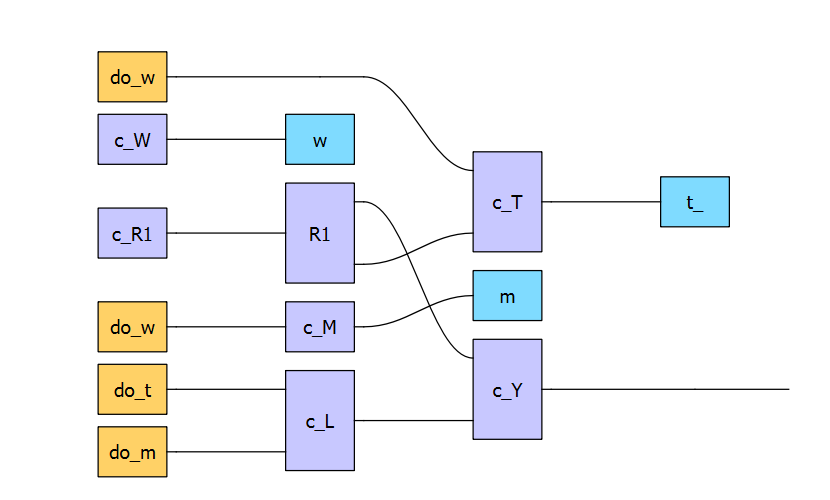
\includegraphics[height=0.5\textwidth]{chyp_example.png}
    \caption{chyp example}
    \label{fig:chyp_example}
\end{figure} 

It is worth noting that the current visualisation pipeline still has some limitations when applied to diagrams produced after the id-cf stage. In particular, Chyp does not currently support a wide range of characters, and unsupported symbols in box labels are automatically replaced with the underscore character ``\_''. This issue becomes especially noticeable in id-cf outputs, where more complex symbolic expressions are involved, and may affect the readability of certain node labels in the exported diagrams.

\chapter{Test and Evaluation}
To verify the correctness and stability of the system implementation, this project adopts a two-tier testing strategy. The first tier is unit testing for each core module, used to check whether local functions meet expected behaviors; the second tier is comparative validation with existing tools, specifically comparing the system's recognition results with the output of the cfid package in R, to confirm the consistency of the overall algorithm on typical inputs. The former mainly focuses on reliability at the implementation level, while the latter primarily focuses on the correctness of the recognition results.

\section{Testing Strategy}
\subsection{Uni-test}
Unit tests mainly cover the key modules throughout the entire pipeline, including ADMG compilation, multi-world construction, counterfactual simplification, R-fragment partitioning, case analysis in ID-CF, and several basic rules in the final expression. For these modules, the focus of testing is not just whether the code can run, but whether they meet the expected structural properties.

For instance, in the ADMG compilation section, the tests check whether bidirectional edges are correctly rootified into explicit latent root nodes, and whether the generated wiring diagram contains the correct number of mechanism nodes and exogenous source nodes. In the multi-world construction section, the tests verify whether all worlds share the same set of exogenous variables, whether mechanism nodes are correctly replicated per world, and whether interventions and observations are properly encoded as sharp states and sharp effects. For simplify-cf, the tests focus on whether discard branches are completely removed, whether sharp effects are correctly separated from fanouts, whether duplicate deterministic boxes are merged, and whether conditional mechanism nodes are replaced with the corresponding Cx nodes. 

In the implementation part of ID-CF, unit tests primarily check the correctness of fragment partitioning and local rewriting. For example, the test for \texttt{find\_r\_fragments} verifies whether the graph is divided into the expected connected components; the tests for \texttt{handle\_case1\_for\_var!} and \texttt{handle\_case2\_for\_var!} respectively construct inputs that meet or do not meet the conditions to check whether the functions return the correct status or correctly throw FAIL when inconsistent. For Step 5, one can test whether parsing of the probability box, summing variable elimination, the drop-do rule, and display mode switching produce the expected expressions.

The purpose of this type of test is to ensure that each local component can operate independently and combine in a predictable manner in the subsequent overall pipeline. Since the entire system involves a large number of graph rewriting and symbol reconstruction steps, unit testing is especially important to prevent local errors from being amplified in later stages.

\subsection{Cross-Tool Validation}
(\cite{cfid_package})
In addition to unit testing of individual modules, the correctness of the overall identification pipeline is further validated through comparison with an existing implementation. Specifically, the output of the proposed system is compared against the results produced by the \texttt{cfid} package in R, which implements counterfactual identification algorithms based on Pearl’s framework.

The purpose of this comparison is to verify semantic equivalence. Due to differences in internal representations, variable naming conventions, and expression formatting, the resulting formulas may differ in ordering or presentation. However, they are considered consistent if they correspond to the same interventional or counterfactual distribution up to algebraic equivalence.

To perform this validation, a set of benchmark queries is constructed, including standard examples such as \texttt{drug}, \texttt{party}, and \texttt{hepar2\_conditional}. For each query, the identification result produced by the system is compared with the output of \texttt{cfid}. In all tested cases where the query is identifiable, both systems return equivalent expressions. In cases where identification is not possible, both systems correctly report failure.

This cross-tool validation provides strong evidence that the implementation faithfully captures the underlying identification logic. It also serves as an end-to-end check of the full pipeline, ensuring that the combination of diagram construction, simplification, recursive identification, and expression reconstruction produces correct results.

\section{Experimental Evaluation}
In addition to verifying correctness through unit testing and cross-tool validation, the performance and scalability of the proposed implementation are further evaluated.

The goal of this evaluation is twofold. First, we compare the runtime performance of the proposed system with an existing implementation, namely the \texttt{cfid} package in R, on a set of benchmark causal models. Second, we investigate how different structural properties of causal graphs affect the performance of the algorithm.

\subsection{Experimental Setup}
All experiments are conducted using the proposed implementation in Julia, built on top of the Catlab library for representing and manipulating wiring diagrams.
The full pipeline includes ADMG compilation, parallel-world construction, counterfactual simplification, recursive identification via the ID-CF algorithm, and final expression reconstruction.

As a baseline, we use the \texttt{cfid} package in R, which implements counterfactual identification algorithms based on Pearl’s framework. This provides a reference point for both correctness and runtime comparison.

The evaluation is carried out on two types of input.
The first type consists of standard benchmark models, including \texttt{drug}, \texttt{party}, and \texttt{hepar2\_conditional}, which are commonly used to test causal identification algorithms.
The second type consists of synthetically generated graph families with controlled structural properties, including chain, fan-in, dense, and heavily confounded graphs (chain\_bi).
These are used to study how the graph structure affects runtime behaviour.

For the synthetic benchmarks, we construct four graph families with controlled structural properties: linear chains, fan-in graphs, dense graphs, and confounded chain graphs with additional bidirected edges. These families are designed to isolate the effect of sparsity, connectivity, and latent confounding on runtime. For each graph of size $n$, the treatment variable is fixed to the first node and the outcome variable to the last node, so that the same counterfactual query pattern is evaluated across all structures.

The timing protocol is aligned across the Julia and R implementations. Both benchmarks use warm runs and report the median over repeated executions. For the Julia implementation, we separately record the time spent in diagram construction, simplification, Step~4, and Step~5, while for the R implementation we record setup time, the time spent inside \texttt{identifiable(...)}, and total runtime. This allows end-to-end comparison through total runtime, while also providing enough internal breakdown to explain performance differences.

All experiments are performed on a standard desktop environment.
Since the focus of this evaluation is on relative performance rather than absolute runtime, hardware-specific optimizations are not considered.

\subsection{Benchmark Comparison}
We first compare the runtime performance of the proposed implementation with the \texttt{cfid} package on a set of standard benchmark models. The goal of this comparison is to evaluate both the efficiency and scalability of the system on representative causal identification tasks.

The selected benchmarks include \texttt{drug}, \texttt{party}, and \texttt{hepar2\_conditional}. (\cite{scutari2010bnlearn})The first two correspond to relatively small causal graphs, while the last one represents a larger and more complex real-world Bayesian network.

\begin{table}[h]
\centering
\begin{tabular}{lccc}
\hline
Case & Julia (ms) & R cfid (ms) & Speedup \\
\hline
drug & 19.85 & 53.37 & $2.69\times$ \\
party & 10.15 & 28.31 & $2.79\times$ \\
hepar2\_conditional & 90.84 & 7812.44 & $86.00\times$ \\
\hline
\end{tabular}
\caption{End-to-end runtime comparison (warm median).}
\label{tab:runtime_total}
\end{table}

Table~\ref{tab:runtime_total} reports the end-to-end runtime comparison. The proposed implementation consistently outperforms \texttt{cfid} across all benchmarks. For small graphs, the speed-up is around 2–3×, while for the larger \texttt{hepar2\_conditional} model, the speed-up exceeds 80×.

\begin{table}[h]
\centering
\resizebox{\textwidth}{!}{%
\begin{tabular}{lcccccccc}
\hline
Example & Julia Build & Julia Simplify & Julia Step4 & Julia Step5 & Julia Setup & Julia Identify & R Identify & Total Speedup \\
\hline
drug   & 0.514 & 16.716 & 2.223 & 0.122 & 17.289 & 2.348 & 47.087 & $2.69\times$ \\
party  & 0.300 & 7.600  & 1.239 & 0.114 & 7.897  & 1.348 & 22.532 & $2.79\times$ \\
hepar2 & 7.958 & 76.454 & 4.926 & 0.294 & 84.924 & 5.265 & 7580.587 & $86.00\times$ \\
\hline
\end{tabular}%
}
\caption{Stage-level runtime breakdown of the Julia implementation and comparison with the R \texttt{cfid} identification time (warm median, repeats = 30, warmups = 5). Here, Julia identify time is defined as \texttt{step4 + step5}, while R identify time corresponds to \texttt{identifiable(...)}.}
\label{tab:benchmark_breakdown}
\end{table}

To better understand the source of this performance difference,
Table~\ref{tab:benchmark_breakdown} reports a fine-grained breakdown of the runtime for the Julia implementation,
together with the identification time of \texttt{cfid}. The results show that the simplification stage accounts for the largest share of the algorithmic cost, while \texttt{step4} and especially \texttt{step5} remain relatively lightweight. In contrast, the R implementation spends most of its time inside the single \texttt{identifiable(...)} call, which encapsulates its recursive identification procedure. This is particularly evident on the \texttt{hepar2\_conditional} benchmark, where the identification stage dominates the overall runtime.

Therefore, the main difference between the two systems is not that one performs preprocessing while the other performs identification, but that the proposed method pushes a substantial part of the identification effort into an explicit diagrammatic simplification stage. This restructuring reduces the complexity of the later symbolic steps and avoids the repeated graph-based computations that dominate the runtime of \texttt{cfid}.

Overall, the results demonstrate that the proposed implementation scales significantly better than \texttt{cfid}, particularly on complex models. This can be attributed to the diagrammatic simplification pipeline, which reduces the complexity of the identification problem before symbolic reconstruction, thereby avoiding repeated graph-based computations.

\subsection{Structural Analysis}
To better understand the performance characteristics of the proposed implementation, we further analyse how different structural properties of causal graphs affect runtime behaviour. In particular, we construct a set of synthetic graph families with controlled structures, which allows me to isolate the impact of sparsity, connectivity, and latent confounding.

The evaluated graph families include chain graphs (chain), fan-in graphs (fanin), dense graphs (dense), and chain graphs with additional bidirected edges representing latent confounding (chain\_bi). These structures represent increasingly complex dependency patterns, from simple linear causality to highly confounded systems.

\begin{table}[h]
\centering
\resizebox{\textwidth}{!}{%
\begin{tabular}{lcccccccc}
\hline
Structure & Build & Simplify & Step4 & Step5 & Julia Total & R Identify & R Total & Speedup \\
\hline
chain     & 2.240 & 149.399 & 10.142 & 0.595 & 162.443 & 901.336 & 963.694 & $5.93\times$ \\
fanin     & 2.994 & 132.847 & 24.679 & 0.463 & 161.653 & 779.834 & 891.755 & $5.52\times$ \\
dense     & 5.569 & 353.262 & 40.791 & 1.047 & 400.669 & 973.114 & 1408.743 & $3.52\times$ \\
chain\_bi & 6.643 & 560.219 & 29.943 & 0.168 & 603.064 & 235.371 & 389.396 & $0.65\times$ \\
\hline
\end{tabular}%
}
\caption{Runtime comparison across graph structures ($n=32$, warm median). The Julia pipeline is decomposed into build, simplify, and identification stages (Step4+Step5), while R reports identification via \texttt{identifiable(...)}.}
\label{tab:structure_main}
\end{table}

Table~\ref{tab:structure_main} shows the runtime comparison across different graph structures at a fixed size ($n=32$).  The results reveal a clear dependence of performance on graph structure. For sparse structures such as \texttt{chain} and \texttt{fanin}, the proposed method achieves consistent speedups of around $5\times$ over \texttt{cfid}. However, as the graph becomes denser (\texttt{dense}) or contains more bidirected edges (\texttt{chain\_bi}), the advantage decreases and may even reverse.

From the stage-level breakdown, it is evident that the dominant cost in the Julia implementation lies in the \texttt{simplify} stage. While the identification stage (Step4+Step5) remains relatively small across all structures, the cost of simplification grows significantly with graph density and the presence of latent confounding. In contrast, the R implementation spends most of its time inside the \texttt{identifiable(...)} call, which scales poorly with graph size and complexity. This difference indicates that the proposed method shifts a substantial portion of the identification effort into an explicit simplification phase, reducing the cost of subsequent symbolic computation.

\begin{table}[h]
\centering
\begin{tabular}{cccccc}
\hline
$n$ & Julia Total & R Total & Julia Simplify & Julia Step4 & Speedup \\
\hline
8  & 43.140  & 49.125  & 39.447  & 2.909  & $1.14\times$ \\
16 & 66.628  & 137.795 & 57.896  & 5.602  & $2.07\times$ \\
24 & 100.854 & 372.461 & 89.015  & 10.354 & $3.69\times$ \\
32 & 162.443 & 963.694 & 149.399 & 10.142 & $5.93\times$ \\
\hline
\end{tabular}
\caption{Scaling behaviour on chain graphs.}
\label{tab:scaling_chain}
\end{table}

The experimental results demonstrate that the performance of the proposed method is strongly structure-dependent. It performs best on sparse graphs with limited confounding, where simplification effectively reduces problem complexity. However, in graphs with many bi-directed edges, the simplification stage becomes the dominant cost, which may offset the gains in the identification phase.


\subsection{Discussion}
The experimental results provide several important insights into the behaviour of the proposed approach.

First, the evaluation confirms that the implementation achieves both correctness and efficiency. The cross-tool validation shows that the system produces results consistent with the \texttt{cfid} package, while the runtime comparison demonstrates clear performance advantages, especially on larger models.

Second, the results highlight a key design trade-off.
Compared to \texttt{cfid}, which performs most of the computation during recursive identification, the proposed method shifts a significant portion of the workload into an explicit simplification stage, a strategy related to structural reduction techniques in causal inference \cite{tian2002general, shpitser2006identification}. This restructuring reduces the complexity of the identification phase (Step~4 and Step~5), leading to consistently low identification costs across all tested cases.

However, this design also introduces a limitation. As shown in the structural analysis, the cost of the simplification stage increases significantly for graphs with high density or extensive latent confounding. In such cases, the preprocessing overhead may dominate the total runtime and even offset the gains obtained from faster identification.

These observations suggest that the efficiency of the proposed approach is strongly dependent on graph structure, a phenomenon well studied in graphical causal models \cite{spirtes2000causation}. It performs particularly well on sparse graphs, where simplification effectively reduces the problem size, but may become less advantageous when the graph contains many bidirected edges.

Another important advantage of the proposed framework is its ability to provide explicit visualisations of the internal computation process. At each major stage of the pipeline, including ADMG compilation, multi-world construction, and simplification, the system can export the intermediate wiring diagrams into Chyp representations. These diagrams make the structure of the computation transparent, allowing users to directly inspect how variables, interventions, and dependencies are transformed throughout the algorithm. This contrasts with existing implementations, such as texttt{cfid}, where the recognition process is largely opaque and difficult to interpret. The availability of intermediate visualizations improves interpretability and also provides practical tools for debugging and analysing complex recognition tasks.

Finally, the current implementation focuses on clarity and correctness rather than aggressive optimisation. There is considerable potential for improving the performance of the simplification stage, for example by introducing incremental rewriting strategies or avoiding repeated full-graph traversals.

Overall, the results indicate that the diagrammatic approach provides a promising alternative to traditional identification algorithms, combining competitive performance with improved transparency and interpretability.

\chapter{Conclusions and Evaluation}
\section{Project Achievements}
The main objective of this project is to build a counterfactual identifiability analysis framework based on diagrammatic representation and to implement the ID-CF algorithm within this framework. More specifically, the project aims to transform the abstract causal reasoning process into an executable computational workflow, thereby bridging the gap between theory and implementation. These objectives have been successfully achieved.

Primarily, the project has implemented a complete end-to-end process, including ADMG compilation, multiverse construction, counterfactual simplification, R-fragment-based recursive identification, and final expression reconstruction. Each stage aligns with the theoretical structure of the ID-CF algorithm, ensuring the correctness and rigor of the implementation.

In addition, the project demonstrates that the problem of counterfactual identifiability can be expressed and manipulated through combinatorial graph structures. By using wiring diagrams, causal models, interventions, and variable dependencies are modularly represented, making the intermediate steps that are implicit in traditional methods explicitly visible.

Moreover, through unit testing and comparison with the 	\texttt{cfid} package in R, the correctness of the system at the semantic level has been confirmed. In all identifiable test cases, the results of this system are algebraically consistent with existing methods.

Finally, in terms of performance, the system exhibits good scalability across multiple benchmark tests. Experimental results show that on complex models, it can achieve a significant speed-up in runtime compared to the \texttt{cfid} implementation.

\section{Critical Evaluation}
While the project successfully meets its primary goals, it also reveals several important strengths and limitations.

A key strength of the proposed approach is the explicit separation between diagrammatic simplification and identification. By performing structural simplifications before
symbolic reconstruction, the system avoids repeated graph-based computations and achieves a lightweight identification phase. This design leads to improved scalability, especially for sparse graphs.

Another significant advantage is the interpretability of the framework. Unlike existing implementations such as \texttt{cfid}, which mostly operate as black-box programs, the proposed system provides explicit intermediate representations. Through integration with \textbf{Chyp}, the internal structure of the computation can be visualised at each stage, including multiverse construction and fragment rewriting. This greatly enhances transparency, making the system easier to debug and analyse. 

However, this method also has certain limitations. Experimental analysis shows that when the graph structure is relatively dense or contains a large number of potential confounding edges (bi-directed edges), the computational cost of the simplification stage increases significantly and it may even become the main bottleneck of the overall runtime. In this case, the preprocessing overhead may offset the performance advantages brought by the identification stage.

Moreover, the validity of the proposed framework depends on the assumptions encoded in the causal model, including conditions such as causal sufficiency and the correct specification of dependencies \cite{causal-sufficiency}.

In practice, real-world data may be coarse-grained, meaning that fine-grained causal interactions are not explicitly represented,
or that different sources of data provide only partial views of the underlying system. Although latent confounding can be partially represented using bi-directed edges, such abstractions may not fully capture the complexity of hidden dependencies in real-world systems, especially when data arises from heterogeneous sources or under varying conditions \cite{bareinboim2016causal}. As a result, the assumed causal model may fail to accurately reflect the true data-generating process, which can in turn affect the validity of the identified causal effects.

This limitation is well recognised in applied causal inference,
where relying solely on observational data can lead to biased or incomplete conclusions, and triangulation across multiple data sources or methods is often necessary \cite{hammerton2021causal}.
    
From an implementation perspective, the system is designed to emphasise structural clarity and theoretical correspondence rather than low-level performance optimisation. For instance, during the simplification process, there are still cases of repeatedly traversing the graph structure, all of which provide room for subsequent optimisation.

In general, the system is functionally complete and can correctly perform counterfactual identifiability analysis tasks; in terms of design, it also follows good modular principles, clearly mapping the theoretical structure to the program implementation. At the same time, the chosen Julia language and \textbf{Catlab} framework provide good support for graph-structured computation and compositional modelling, making it a reasonable technical choice.

\section{Future Work}
There are several directions in which the project could be extended if additional time were available.

In terms of improving the current implementation, the most immediate priority would be to optimise the simplification stage. This could involve developing incremental rewriting 
strategies, avoiding repeated full-graph scans, or introducing more efficient data structures for representing wiring diagrams.

Another direction is to extend the framework to support a broader class of queries. Currently, the implementation focuses on standard counterfactual identification tasks. Future work could include more complex query types, richer intervention patterns, or integration with probabilistic inference engines.

From a usability perspective, the visualisation component could be further developed into an interactive tool, allowing users to explore intermediate diagrams dynamically. This would enhance the practical value of the system for both research and teaching.
The limitations of the \textbf{chyp} tool are quite significant. If there is enough time, one could develop a new visualization tool specifically for interactive display of string diagrams, capable of representing all structures in a string diagram in detail, as well as enabling dragging, splicing, and even intervention operations.

Finally, there is potential to connect this framework with machine learning systems, for example by integrating it into causal representation learning pipelines or reinforcement learning environments.

It is important to note that these extensions go beyond the original scope of the project, which focuses on establishing a correct and efficient implementation of the ID-CF pipeline. 
The current work successfully achieves its stated goals, while the above directions represent natural extensions.

\section{Conclusion}
In conclusion, this project demonstrates that the string-diagram-based representation approach can not only provide a clear theoretical framework for counterfactual identifiability, but also support efficient computational implementation. By transforming the causal reasoning process into an operable graph structure transformation, this system achieves good performance and interpretability while maintaining theoretical rigour. This provides new ideas and possibilities for the integration of causal reasoning, categorical methods, and computational systems.


\nocite{10.1093/biomet/82.4.669}
\nocite{tikka2021cfid}
\nocite{huang2006completeness}
\nocite{Fritz_2020}
\nocite{koller2009probabilistic}

\bibliographystyle{IEEEtran}
\bibliography{ref}

\appendix

\chapter{System/User Manual}
\label{app:system}

This appendix provides the technical information required to install, run, reproduce, and extend the implementation. 
The full source code is available at:

\begin{center}
\texttt{https://github.com/GrayratA/FYP}
\end{center}

\section{Repository Structure}

The repository is organised as follows:

\begin{itemize}
    \item \texttt{src/}: Core Julia implementation. This includes ADMG compilation, Bayesian-network import, counterfactual simplification, ID-CF, Chyp export, and utility functions.
    \item \texttt{src/123.ipynb} and \texttt{src/test.ipynb}: Development-time notebooks used during testing. These are not required for running the system.
    \item \texttt{test/}: Julia unit test suites for the main modules, including ADMG compilation, simplification, and ID-CF.
    \item \texttt{net/}: Bayesian network structure files, including examples such as \texttt{hepar2.net}.
    \item \texttt{tools/}: Helper scripts, including utilities for converting Bayesian-network structures to ADMG representations.
    \item \texttt{comparisons/}: Benchmark scripts and comparison artefacts.
    \item \texttt{comparisons/runtime/}: Main Julia versus R \texttt{cfid} runtime benchmarks.
    \item \texttt{comparisons/runtime/structural\_tests/}: Structural scaling benchmark scripts, raw data, CSV generation scripts, and profiling outputs.
    \item \texttt{trace/}: Intermediate trace artefacts, including Chyp files generated during diagrammatic visualisation.
\end{itemize}

\section{Installation}

The implementation is written in Julia and uses the package environment specified by \texttt{Project.toml} and \texttt{Manifest.toml}. 
The R package \texttt{cfid} is only required for running the comparison benchmarks.

The required software is:

\begin{itemize}
    \item Julia, using the project environment supplied in the repository;
    \item R with the \texttt{cfid} package installed, if R-side benchmarks are required.
\end{itemize}

After cloning the repository, Julia dependencies can be installed with:

\begin{verbatim}
julia --project=. -e "using Pkg; Pkg.instantiate()"
\end{verbatim}

\section{Running Tests}

The full Julia test suite can be run using:

\begin{verbatim}
julia --project=. test/runtest.jl
\end{verbatim}

These tests cover the main components of the pipeline, including ADMG compilation, counterfactual simplification, and ID-CF.

\section{Main API}

The main entry point of the system is:

\begin{verbatim}
identify_counterfactual(...)
\end{verbatim}

This function performs the full counterfactual identification pipeline. It builds the SCM and multiverse diagram from a graph and a set of queries, runs simplification, applies Step 4 and Step 5 of the ID-CF implementation, and returns the identifiability status together with formula output and diagnostic information.

The core files can be loaded as follows:

\begin{verbatim}
using Catlab

include("src/admg_compile.jl")
include("src/simplify_cf.jl")
include("src/id_cf.jl")
include("src/bn_import.jl")     # optional, for reading .bif/.net files
include("src/chyp_export.jl")   # optional, for trace_dir visualisation output
\end{verbatim}

The function \texttt{run\_cf\_pipeline(...)} is an alias of \texttt{identify\_counterfactual(...)}.

\section{Output Fields}

The result object returned by \texttt{identify\_counterfactual} includes the following important fields:

\begin{itemize}
    \item \texttt{res.identifiable}: Whether Step 4 succeeds.
    \item \texttt{res.formula\_available}: Whether Step 5 successfully produces formula text.
    \item \texttt{res.raw\_tex}: The raw reconstructed formula.
    \item \texttt{res.simplified\_tex}: The simplified formula.
    \item \texttt{res.data\_tex}: The data-mode rewritten formula, when applicable.
    \item \texttt{res.failure\_stage}: The failed stage, or \texttt{nothing} if no failure occurs. Possible values include \texttt{:build}, \texttt{:simplify}, \texttt{:step4}, and \texttt{:step5}.
    \item \texttt{res.error}: Error message when failure occurs.
    \item \texttt{res.step3\_blockers}: Unabsorbed lambda boxes before Step 4.
    \item \texttt{res.trace\_paths}: Paths of written \texttt{.chyp} files when \texttt{trace\_dir} is enabled.
    \item \texttt{res.timings\_ms}: Runtime breakdown by stage.
\end{itemize}

\section{Runtime Benchmarks}

The main runtime comparison between the Julia implementation and the R \texttt{cfid} package can be reproduced using:

\begin{verbatim}
julia --project=. comparisons/runtime/julia_benchmark.jl 30 5
Rscript comparisons/runtime/r_cfid_benchmark.R 30 5
\end{verbatim}

Further benchmark details, including field definitions and timing alignment notes, are provided in:

\begin{verbatim}
comparisons/runtime/README.md
\end{verbatim}

\section{Structural Scaling Benchmarks}

Structural scaling experiments can be reproduced using the scripts in:

\begin{verbatim}
comparisons/runtime/structural_tests/
\end{verbatim}

For example:

\begin{verbatim}
julia comparisons/runtime/structural_tests/scripts/struct_scaling_julia.jl 4 2 8,16,24,32

Rscript comparisons/runtime/structural_tests/scripts/struct_scaling_r.R 4 2 8,16,24,32
\end{verbatim}

The generated raw outputs can then be converted into CSV format using the provided PowerShell script:

\begin{verbatim}
pwsh -File comparisons/runtime/structural_tests/scripts/make_struct_csv.ps1 -Tag r4w2
\end{verbatim}

\section{Utility Scripts}

The repository includes a utility for converting Bayesian network structure files into ADMG Julia literals:

\begin{verbatim}
julia --project=. tools/import_bn_to_admg.jl <input.bif|input.net> [output.jl] [model_name]
\end{verbatim}

This is useful when importing benchmark models such as \texttt{hepar2.net}.

\section{Extending the System}

The system is organised modularly. Future developers may extend it in the following ways:

\begin{itemize}
    \item Add new graph-import formats in \texttt{src/bn\_import.jl}.
    \item Add or optimise diagrammatic rewriting rules in \texttt{src/simplify\_cf.jl}.
    \item Extend Step 4 or Step 5 logic in \texttt{src/id\_cf.jl}.
    \item Improve or replace the Chyp exporter in \texttt{src/chyp\_export.jl}.
    \item Add new benchmark families in \texttt{comparisons/runtime/structural\_tests/}.
\end{itemize}


\chapter{Diagrammatic Visualisation Example: HEPAR2}
\label{app:hepar2_vis}

Due to some constraints (The visual chart in chyp is not convenient to show with screenshots (it's too large).), the full set of diagrammatic visualisations for the \texttt{HEPAR2} example is not included directly in this report. 
Instead, all intermediate wiring diagrams generated during the pipeline are provided in the project repository.

Specifically, the visualisation outputs can be found in:

\begin{center}
\texttt{trace/HEPAR2/}
\end{center}

This directory contains a sequence of \texttt{.chyp} files corresponding to different stages of the pipeline:

\begin{itemize}
    \item \texttt{01\_base\_scm.chyp}: the compiled structural causal model,
    \item \texttt{02\_multiverse.chyp}: the parallel-world construction,
    \item \texttt{03--06\_simplify*.chyp}: intermediate simplification steps,
    \item \texttt{07\_step4.chyp}: the final structure before expression reconstruction.
\end{itemize}

To view these visualisations, the \textbf{Chyp} tool must be installed. 
Chyp is an interactive environment for inspecting and manipulating string diagrams, available at:

\begin{center}
\texttt{https://github.com/akissinger/chyp}
\end{center}

After installing Chyp, the \texttt{.chyp} files can be opened directly to explore the diagrammatic structure of each stage.

These visualisations provide a complete trace of how the counterfactual identification pipeline transforms the initial model into a simplified structure suitable for symbolic reconstruction. 
This external representation complements the experimental results presented in Chapter~5, and allows the internal computation process to be inspected interactively, which would not be feasible within the page constraints of this report.


\chapter{Full Test Results: R cfid vs Julia}
\label{app:test_result}
\section{Full Test Results}

This appendix presents the complete experimental results for all configurations.
All tables are directly generated from the original CSV files to ensure reproducibility
and to avoid manual transcription errors.

\subsection{Combined Results (Julia vs R)}

This table reports the overall runtime comparison between the Julia implementation
and the R baseline across different structural settings and problem sizes.

\begin{center}
\resizebox{\textwidth}{!}{
\pgfplotstabletypeset[
    col sep=comma,
    string type,
    every head row/.style={
        before row=\toprule,
        after row=\midrule
    },
    every last row/.style={
        after row=\bottomrule
    }
]{test_result/struct_combined_r4w2.csv}
}
\end{center}

\subsection{Julia Implementation Breakdown}

This table provides a detailed breakdown of runtime components for the Julia implementation,
including setup, identification, simplification, and other intermediate steps.

\begin{center}
\resizebox{\textwidth}{!}{
\pgfplotstabletypeset[
    col sep=comma,
    string type,
    every head row/.style={
        before row=\toprule,
        after row=\midrule
    },
    every last row/.style={
        after row=\bottomrule
    }
]{test_result/struct_julia_r4w2.csv}
}
\end{center}

\subsection{R Implementation Breakdown}

This table shows the corresponding runtime breakdown for the R implementation,
used as a baseline for comparison.

\begin{center}
\resizebox{\textwidth}{!}{
\pgfplotstabletypeset[
    col sep=comma,
    string type,
    every head row/.style={
        before row=\toprule,
        after row=\midrule
    },
    every last row/.style={
        after row=\bottomrule
    }
]{test_result/struct_r_r4w2.csv}
}
\end{center}

\chapter{Project Plan}
\documentclass[12pt,a4paper]{article}
\usepackage{geometry}
\geometry{a4paper,margin=2.5cm}
\usepackage{setspace}
\usepackage{titlesec}
\usepackage{enumitem}
\usepackage{graphicx}
\usepackage{hyperref}
\linespread{1.25}

\titleformat{\section}{\large\bfseries}{\thesection}{1em}{}
\titleformat{\subsection}{\normalsize\bfseries}{\thesubsection}{1em}{}
\setlist[itemize]{leftmargin=2em}

\begin{document}

% ==========================
%   TITLE PAGE
% ==========================
\begin{center}
    \vspace*{1cm}
    {\LARGE \textbf{UCL Final Year Project Plan}}\\[1.5em]
    {\Large \textbf{Project Title:}}\\[0.5em]
    {\large Categorical Implementation of Counterfactual Identification Algorithms in String Diagrams}\\[2em]
    \begin{tabular}{rl}
        \textbf{Supervisor:} & Prof.\ Fabio Zanasi \\
        \textbf{External Supervisor:} & N/A \\
        \textbf{Degree Programme:} & MEng Computer Science \\
        \textbf{Date:} & October 2025 \\
    \end{tabular}
\end{center}


\newpage

% ==========================
%   PROJECT SECTIONS
% ==========================

\section{Project Title}
Categorical Implementation of Counterfactual Identification Algorithms in String Diagrams

\section{Aims and Objectives}

\subsection*{Aim}
The project aims to establish a formal and computational framework based on string diagrams for analysing the identifiability of causal and counterfactual expressions.

Building upon recent advances in category-theoretic causal reasoning(\cite{lorenz2023causal}), the project will study and implement core identifiability algorithms — particularly simplify-cf and id-cf — and realise them categorically within the AlgebraicJulia framework.

The core idea of this project is to use string diagrams as a unified graphical and semantic representation framework.
They can not only make explicit the compositional structure of causal dependencies but also serve as computational objects that can be manipulated algorithmically to perform symbolic reasoning over causal and counterfactual identifiability.
By encoding both the syntax and semantics of these diagrams categorically within AlgebraicJulia, the project enables automated reasoning about interventions, observable distributions, and counterfactual relationships.

The project will begin by formalising the string diagrammatic structures used to represent parallel-worlds models and counterfactual worlds.
It will then implement the simplify-cf and id-cf algorithms as compositional transformations on these diagrams, enabling symbolic simplification and identifiability checking directly at the level of diagrammatic semantics.

Although the initial focus is on counterfactual identifiability, the framework is designed to generalise naturally to causal identifiability in general.

In addition, the project will explore integrating the implementation with a lightweight graphical interface inspired by Chyp (https://github.com/akissinger/chyp
), enabling visual diagram editing, interactive causal reasoning, and real-time visualisation of string-diagram transformations.

\subsection*{Objectives}
To achieve the above aim, the project will pursue the following objectives:
\begin{enumerate}
    \item Explore relevant literature on causal inference, counterfactual reasoning, and category-theoretic approaches.
    The exploration will focus on how string diagrams and symmetric monoidal categories can be used as graphical and compositional tools for representing causal structures and reasoning about interventions. It will also include a detailed study of the two key counterfactual algorithms — simplify-cf and id-cf — to understand their theoretical foundations and graphical semantics.
    \item Learn the Julia programming language and become familiar with using AlgebraicJulia (particularly Catlab.jl) to construct and manipulate counterfactual and causal models. This stage will focus on building the necessary technical background to encode diagrammatic structures and to prepare for the later implementation of identifiability algorithms.
    \item Implement the \textit{simplify-cf} algorithm as a compositional rewriting process on string diagrams for symbolic simplification of counterfactual queries.
    \item Implement the \textit{id-cf} algorithm to recursively determine counterfactual identifiability and produce equivalent expressions in observable or interventional terms.
    \item Validate the implementation through canonical examples from the literature (e.g., those discussed by Shpitser and Pearl \cite{shpitser2008complete} ), ensuring that the algorithms reproduce the expected causal and counterfactual identifiability results. Additionally, perform systematic testing on synthetic and edge-case scenarios to evaluate the implementation’s correctness, robustness to structural variations, and computational efficiency under different graph configurations.
    \item Generalise the developed framework to handle general causal identifiability problems beyond counterfactuals.
    \item Explore integration with a lightweight graphical interface inspired by \textit{Chyp} to enable visual causal reasoning and interactive diagram manipulation.
\end{enumerate}

\subsection*{Deliverables}
The following deliverables are expected from this project:
\begin{enumerate}
    \item \textbf{Algorithmic Implementation:}
    A working prototype implementing the \textit{simplify-cf} and \textit{id-cf} algorithms in the \textit{AlgebraicJulia} framework, operating directly on string-diagrammatic representations of causal models for automated simplification and identifiability checking.

    \item \textbf{Formal Specification and Documentation:}
    Detailed documentation of the categorical and diagrammatic semantics underlying the implementation, including formal definitions, data structures, and transformation rules.

    \item \textbf{Testing and Evaluation Suite:}
    A comprehensive set of test cases including canonical examples from the literature (e.g., Shpitser and Pearl~\cite{shpitser2008complete}) and synthetic edge-case scenarios, used to assess correctness, robustness, and computational efficiency.

    \item \textbf{Example Library:}
    A curated library of causal and counterfactual diagrams encoded in AlgebraicJulia, demonstrating the operation of the algorithms across different model structures.

    \item \textbf{Final Technical Report:}
    A full written report covering theoretical background, implementation details, testing methodology, results, and discussion of limitations and future work.


    \item \textbf{Visual Interface Prototype:}
    An exploratory GUI or interactive front-end (inspired by \textit{Chyp}) for diagrammatic causal reasoning, integrated with the AlgebraicJulia backend.
\end{enumerate}


\subsection*{Work Plan}

The project will be conducted from October 2025 to March 2026, following a structured progression from theoretical foundation to implementation, evaluation, and visualization. Each stage will deliver concrete outcomes aligned with the objectives and deliverables described above.

\textbf{October 2025 – Literature search and Theoretical Foundation}

Conduct an in-depth literature search on causal inference, counterfactual reasoning, and category-theoretic frameworks for causal modelling (e.g., Lorenz and Tull~\cite{lorenz2023causal}, Shpitser and Pearl~\cite{shpitser2008complete}).  
Study the role of string diagrams in representing causal dependencies and familiarise with the AlgebraicJulia ecosystem (particularly \textit{Catlab.jl}) for categorical modelling.

\textbf{November – Mid December 2025 – Implementation on Specific Examples}

Design and formalise the string-diagrammatic representation for small-scale counterfactual models.  
Implement preliminary prototypes of the \textit{simplify-cf} and \textit{id-cf} algorithms on isolated examples to verify their correctness and consistency with category-theoretic semantics.

\textbf{Mid December 2025 – Mid January 2026 – Generalisation and Full Algorithm Implementation}

Extend the initial prototype to handle arbitrary causal diagrams, generalising the framework to a broader class of counterfactual structures.  
Integrate \textit{simplify-cf} and \textit{id-cf} into a unified compositional pipeline capable of performing automated simplification and identifiability checking on general diagrams.

\textbf{Mid January – Mid February 2026 – Testing and Evaluation}

Test the complete implementation on canonical examples from the literature (e.g., those discussed by Shpitser and Pearl~\cite{shpitser2008complete}) and on synthetic diagrams designed to explore edge cases.  
Evaluate the implementation’s correctness, robustness to structural variations, and computational efficiency.

\textbf{Mid February – Early March 2026 – Visual Interface Prototype}

Develop a lightweight visual interface prototype, inspired by \textit{Chyp}, that connects to the AlgebraicJulia backend.  
This prototype will enable interactive visualization and manipulation of string diagrams, allowing users to inspect compositional transformations and identifiability outcomes visually.

\textbf{March 2026 – Final Report}

Prepare the final technical report, including theoretical background, implementation details, evaluation results, and future work.  




\chapter{Interim Report}
\documentclass[12pt,a4paper]{article}
\usepackage{geometry}
\geometry{a4paper,margin=2.5cm}
\usepackage{setspace}
\usepackage{titlesec}
\usepackage{enumitem}
\usepackage{graphicx}
\usepackage{hyperref}
\linespread{1.25}

\titleformat{\section}{\large\bfseries}{\thesection}{1em}{}
\titleformat{\subsection}{\normalsize\bfseries}{\thesubsection}{1em}{}
\setlist[itemize]{leftmargin=2em}

\begin{document}

% ==========================
%   TITLE PAGE
% ==========================
\begin{center}
    \vspace*{1cm}
    {\LARGE \textbf{UCL Final Year Project interim report}}\\[1.5em]
    {\Large \textbf{Project Title:}}\\[0.5em]
    {\large Categorical Implementation of Counterfactual Identification Algorithms in String Diagrams}\\[2em]
    \begin{tabular}{rl}
        
        \textbf{Supervisor:} & Prof.\ Fabio Zanasi \\
        \textbf{External Supervisor:} & N/A \\
        \textbf{Degree Programme:} & MEng Computer Science \\
        \textbf{Date:} & Jan 2026 \\
    \end{tabular}
\end{center}


\newpage
\section{Introduction}

Counterfactual reasoning is a fundamental component of causal inference, enabling the evaluation of hypothetical scenarios such as how outcomes would change under alternative 
interventions. 
While Structural Causal Models (SCMs) provide a well-established semantic foundation for 
counterfactuals, determining whether a counterfactual query is identifiable from observed 
and interventional data remains a non-trivial algorithmic problem, especially in the 
presence of latent confounding.

Recent work by Robin Lorenz and Sean Tull(\cite{lorenz2023causal}) introduced a compositional and diagrammatic 
approach to counterfactual identification based on Acyclic Directed Mixed Graphs (ADMGs)
and rooted wiring diagrams. 
Their \textit{id-cf} algorithm offers a complete procedure for identifying general 
counterfactual queries by decomposing causal graphs into independent fragments and 
systematically rewriting them into probability expressions. 
However, the original work focuses on theoretical development and does not provide a 
fully executable implementation.

This project aims to implement an end-to-end realisation of the \textit{id-cf} algorithm. 
Given an ADMG and a multi-world counterfactual query, the system automatically constructs 
a categorical wiring diagram, applies diagrammatic simplification and fragment-based 
rewriting, and ultimately produces an explicit sum--product probability expression when 
the query is identifiable. 
The implementation is carried out in Julia using the Catlab framework, with a focus on 
compositionality, modularity, and faithful alignment with the theoretical semantics.


\section{Current process summary}
So far, my project has achieved substantial progress across all core technical components. The first major milestone completed was the development of a generalisation and compilation framework for arbitrary acyclic directed mixed graphs (ADMGs). Users can now input any ADMG together with a specification of counterfactual worlds, interventions, or conditioning operations. The system automatically compiles this abstract causal structure into a corresponding rootified wiring diagram expressed in Catlab.jl. This required implementing a systematic translation from mixed-graph structure to category-theoretic primitives, including mechanism boxes, bidirected confounding via root nodes, and world-indexed variable instantiations. As a result, the entire pipeline is now independent of fixed examples and works uniformly for any valid ADMG.

Building on the compiled diagrams, I then completed the full implementation of the \textit{simplify-cf} algorithm, which rewrites counterfactual diagrams into a normalised and canonical form. This involved encoding graphical identities such as propagation of sharp states/effects, elimination of redundant structure, handling of parallel-world models, and composition of mechanisms according to the categorical semantics. The module has been thoroughly tested on non-trivial counterfactual examples from the literature and produces diagrams that exactly match the theoretical expectations. This component forms the foundation for the subsequent identification procedure.

The most technically demanding part of the project has been the  implementation of the \textit{id-cf} counterfactual identification algorithm, particularly its case-based rewrites within each R-fragment. For every variable $X$, the system determines whether the mechanism $c_X$ lies inside the fragment (\textbf{Case 1}) or outside (\textbf{Case 2}), and then performs the exact structural rewrite prescribed by the algorithm. In \textbf{Case 1a}, where the output of $c_X$ connects only to external fragments or final outputs and no additional $X$-type inputs exist inside the fragment, no modification is required; in \textbf{Case 1b}, where the output wire of $c_X$ is composed with some sharp effect x and any other wires of type X inside the fragment all have the state x fed into them, the diagram must be rewritten so that all internal uses of $X$ are consistently supplied by the local $c_X$, following the rules in report. In \textbf{Case 2a}, all $X$-inputs originate from a single external $c_X$ via fan-out, which again requires no rewrite; whereas in \textbf{Case 2b}, all $X$-inputs come from the same sharp state (e.g.\ $\mathrm{do}(X)$), and the fragment must be rewritten by merging these state inputs into a single source, following the rules in report. After all variables have passed their Case analysis and the appropriate rewrites are applied, replaces the entire R-fragment with a probability box 
\[
P(C_l, F^{\mathrm{out}}_l;\ \mathrm{do}(D_l),\ \mathrm{do}(F^{\mathrm{in}}_l)),
\]
where the sets $C_l$, $F^{\mathrm{out}}_l$, $D_l$ and $F^{\mathrm{in}}_l$ are automatically extracted from the diagram. This completes the essential structural transformation required for counterfactual identification and enables the algorithm to map simplified wiring diagrams into fully identified probabilistic expressions.

\section{Remaining work}

\subsection{Completion of the Final Output Stage.}
The first remaining task is to complete the final stage of the \textit{id-cf} algorithm, namely generating the explicit sum--product probability expression from the final wiring diagram. This requires extracting all fragment-level probability factors of the form 
\[
P(C_l, F^{\mathrm{out}}_l \,;\, \mathrm{do}(D_l), \mathrm{do}(F^{\mathrm{in}}_l)),
\]
and assembling them into a single symbolic expression that matches the structure specified in the original identification algorithm. Once implemented, this component will produce the complete analytic counterfactual estimand, representing the final output of the entire \textit{id-cf} pipeline and enabling direct mathematical or computational evaluation.

\subsection{Testing and Validation.}
The second outstanding task is to construct a systematic and comprehensive test suite. This will include ADMGs and counterfactual queries collected from the literature, classic examples used widely across causal inference papers as well as a variety of edge cases and custom synthetic tests. By validating the outputs of both \textit{simplify-cf} and \textit{id-cf} across a broad range of graph structures and counterfactual scenarios, the aim is to ensure the correctness, robustness, and stability of the entire identification pipeline.

\subsection{Comparison with Existing Tools}
The third task is to conduct a systematic comparison with state-of-the-art counterfactual identification tools, such as the R package \textit{cfid} (implementing the ID*/IDC* algorithms), the Python library Y0, and other causal-identification frameworks. The comparison will cover aspects including: expressive power (e.g.\ support for parallel-world 
representations), compositionality, generality with respect to ADMGs, and computational performance. Through these criteria, the advantages and limitations of the present project will be identified, and future directions for improvement will become clearer.

\subsection{Development of a Visualisation Component}
The final planned task is to develop a visualisation module that can present the wiring diagrams, R-fragment decompositions, and intermediate rewrites produced by both \textit{simplify-cf} and \textit{id-cf}. The preferred solution is to integrate the tool with \textit{Chyp}, which provides high-quality string diagram rendering and supports interactive exploration of categorical structures. If full integration with \textit{Chyp} proves technically challenging, alternative approaches based on Catlab's internal visualisation facilities or custom Julia-based diagram rendering will be explored. A visualisation component would significantly enhance interpretability of the algorithm, facilitate debugging, and provide clearer insight into how the identification procedure operates on different fragments and graphical configurations.


% \end{document}



\end{document}

